\documentclass[12pt,oneside]{uhthesis}
\usepackage{subfigure}
\usepackage[ruled,lined,linesnumbered,titlenumbered,algochapter,onelanguage]{algorithm2e}
\usepackage{amsmath}
\usepackage{amssymb}
\usepackage{amsbsy}
\usepackage{caption,booktabs}
\captionsetup{ justification = centering }
%\usepackage{mathpazo}
\usepackage{float}
\setlength{\marginparwidth}{2cm}
\usepackage{todonotes}
\usepackage{listings}
\usepackage{xcolor}
\usepackage{changepage}
\usepackage{multicol}
\usepackage{graphicx}
\floatstyle{plaintop}
\restylefloat{table}
\addbibresource{Bibliography.bib}
% \setlength{\parskip}{\baselineskip}%
\renewcommand{\tablename}{Tabla}
\renewcommand{\listalgorithmcfname}{Índice de Algoritmos}
%\dontprintsemicolon
\SetAlgoNoEnd

\definecolor{codegreen}{rgb}{0,0.6,0}
\definecolor{codegray}{rgb}{0.5,0.5,0.5}
\definecolor{codepurple}{rgb}{0.58,0,0.82}
\definecolor{backcolour}{rgb}{0.95,0.95,0.92}

\lstdefinestyle{mystyle}{
    backgroundcolor=\color{backcolour},   
    commentstyle=\color{codegreen},
    keywordstyle=\color{purple},
    numberstyle=\tiny\color{codegray},
    stringstyle=\color{codepurple},
    basicstyle=\ttfamily\footnotesize,
    breakatwhitespace=false,         
    breaklines=true,                 
    captionpos=b,                    
    keepspaces=true,                 
    numbers=left,                    
    numbersep=5pt,                  
    showspaces=false,                
    showstringspaces=false,
    showtabs=false,                  
    tabsize=4
}

\lstset{style=mystyle}

\title{Extracción y estudio de la argumentación en la prensa cubana}
\author{\\\vspace{0.25cm}Luis Ernesto Ibarra Vázquez}
\advisor{\\\vspace{0.25cm}MsC. Damian Valdés Santiago}
\degree{Licenciado en Ciencia de la Computación}
\faculty{Facultad de Matemática y Computación}
\date{Fecha\\\vspace{0.25cm}\href{https://github.com/luisoibarra/thesis}{github.com/luisoibarra/thesis}} % TODO PREGUNTA EL repo de la tesis o el de la implementación?
\logo{Graphics/uhlogo}
\makenomenclature

\renewcommand{\vec}[1]{\boldsymbol{#1}}
\newcommand{\diff}[1]{\ensuremath{\mathrm{d}#1}}
\newcommand{\me}[1]{\mathrm{e}^{#1}}
\newcommand{\pf}{\mathfrak{p}}
\newcommand{\qf}{\mathfrak{q}}
%\newcommand{\kf}{\mathfrak{k}}
\newcommand{\kt}{\mathtt{k}}
\newcommand{\mf}{\mathfrak{m}}
\newcommand{\hf}{\mathfrak{h}}
\newcommand{\fac}{\mathrm{fac}}
\newcommand{\maxx}[1]{\max\left\{ #1 \right\} }
\newcommand{\minn}[1]{\min\left\{ #1 \right\} }
\newcommand{\lldpcf}{1.25}
\newcommand{\nnorm}[1]{\left\lvert #1 \right\rvert }
\renewcommand{\lstlistingname}{Ejemplo de código}
\renewcommand{\lstlistlistingname}{Ejemplos de código}

\begin{document}

\frontmatter
\maketitle

\begin{dedication}
    Dedicación
\end{dedication}
\begin{acknowledgements}
    Agradecimientos
\end{acknowledgements}
\begin{opinion}
La lingüística computacional es una rama multidisciplinaria que procesa grandes 
cantidades de textos escritos. La tesis presentada por Luis Ernesto Ibarra Vázquez 
propone un algoritmo basado en modelos de aprendizaje automático para la segmentación 
y clasificación de enunciados argumentativos en textos de la sección “Cartas a la Dirección” 
del periódico \emph{Granma}.

La tesis se ubica en el marco de un proyecto \emph{Dinámicas sociales, políticas y económicas en el 
discurso público en Cuba de principio del siglo XXI: estudios de CORESPUC}, asociado al Programa 
Nacional de Ciencia y Técnica “Las Ciencias Sociales y las humanidades. Desafíos ante la estrategia 
de desarrollo de la sociedad cubana”, Código PN223LH011-011, Ministerio de Ciencia, Tecnología y 
Medio Ambiente (CITMA), Cuba, 2021-2023.

Por ello, Luis Ernesto tuvo que estudiar la materia referida, que no está incluida en el currículo 
de la carrera y trabajó mostrando creatividad, disciplina, entrega y rigor. Deseo destacar su 
profundización en el estudio computacional de la argumentación y la proposición de soluciones de 
software útiles para el análisis de enunciados argumentativos en español.

La investigación realizada por el estudiante incluyó diversos corpus en idioma inglés con 
diferentes anotaciones de la argumentación que se usaron para el entrenamiento de modelos de 
aprendizaje automático proyectivos para clasificar los enunciados argumentativos en español, a 
partir del conocimiento de la anotación en idioma inglés. Se compararon varios modelos y el mejor 
fue utilizado para la clasificación de enunciados de las Cartas a la Dirección del periódico Granma. 
Este trabajo es un primer paso positivo en el estudio automático de la argumentación de nuestra variante 
del español y llevará una posterior revisión por lingüistas. Dicho corpus anotado será importante para la 
realización de análisis sociolingüísticos del corpus donde la argumentación es una variable de interés para 
el proyecto CORESPUC.

Durante el desarrollo del trabajo, Luis Ernesto demostró habilidades para el trabajo con la bibliografía y 
creatividad para proponer soluciones a problemas de implementación, entre otras competencias de programación 
en el lenguaje Python y sus diversos \emph{frameworks}. Así, se logró cumplir el objetivo de esta tesis.

Por tanto, considero que al estudiante Luis Ernesto Ibarra Vázquez debe otorgársele la máxima calificación 
(5 puntos, Excelente), y estoy seguro que en el futuro Luis Ernesto se desempeñará como un excelente profesional 
de la Ciencia de la Computación.

\begin{flushright}
\includegraphics[scale=0.2]{Graphics/firma.jpg}\\
MSc. Damian Valdés Santiago\\
21 de noviembre de 2022    
\end{flushright}

\end{opinion}
\begin{resumen}
	Resumen en español
\end{resumen}

\begin{abstract}
	Resumen en inglés
\end{abstract}
\tableofcontents
\listoffigures
% \listoftables
% \listofalgorithms
\lstlistoflistings

\mainmatter

\chapter*{Introducción}\label{chapter:introduction}
\addcontentsline{toc}{chapter}{Introducción}

% Introducción a la teoría de la argumentación

La teoría de la argumentación es el estudio interdisciplinario de cómo las conclusiones
pueden ser apoyadas o socavadas por premisas a través de razonamiento lógico [\cite{wiki-arg-theory}] .
Esta es usada en varios aspectos de la vida como en las negociaciones, debates públicos, publicaciones
científicas, enseñanza, leyes. Sobre este marco teórico es sobre donde se realiza el diseño y análisis de 
modelos computacionales que ayudan al procesamiento de los grandes volúmenes de datos existentes.

En la actualidad es necesario tener acceso a la información necesaria
de forma rápida y simple. Esto no siempre es posible dado la gran cantidad de información existente y
que es generada en cada momento. En caso de tener una vía de acceder a esta se podrían realizar acciones
con mayor rapidez y calidad. Con la argumentación se podría hacer explícitas las razones de las personas 
al afirmar algo sobre un tema teniendo así su punto de vista individual, y con suficientes personas, colectivo.

% Presentación de la problemática

La Extracción de Argumentos (EA) es la rama del Procesamiento de Lenguaje Natural encargada de formularizar
y modelar dicho problema. Los modelos existentes generalmente se encargan de
extraer y clasificar las componentes argumentativas y sus relaciones de una fuente no estructurada de 
texto, capturando un proceso de razonamiento y argumentación en su estructura final. Los métodos
de realizar este procedimiento varían en dependencia de las características en que se trabaja y el objetivo
a que se quiere llegar. Entre los métodos usados se pueden mencionar métodos ad-hoc basados en gramáticas,
que aprovechan atributos del texto como partes de la oración y entidades nombradas, que codifican diferentes 
patrones argumentativos [\cite{dykes2020reconstructing}]. Dicho enfoque requiere de trabajo 
humano para la creación de una gramática que permita resultados satisfactorios. Este tipo de enfoque
generalmente sacrifica recobrado por precisión y no permite una generalización del problema, contribuyendo
a no ser muy escalable.

Existen método basados en técnicas de aprendizaje de máquina para modelar y resolver dicho problema.
Estos métodos están divididos en diferentes vertientes de acuerdo a cómo procesan los datos. Uno de ellos lo realiza por
etapas, en el cual en cada una se resuelve independientemente los subproblema y la salida de la etapa 
anterior es entrada a la etapa siguiente. Las etapas en que generalmente se divide el problema
son, separación de unidades argumentativas y no argumentativas, clasificación de las unidades 
argumentativas y la identificación de estructuras argumentativas [\cite{stab2014identifying}].
Este enfoque trae consigo una modularidad elevada al resolver las tareas de manera independiente, pero
tiene la desventaja que los errores de etapas anteriores son pasados a las siguientes y además los algoritmos
usados no ven todo el contexto del texto pudiendo perder características que permitirían un mejor resultado.
Otro enfoque usado son los llamados end-to-end, en estos el modelo entrenado aprende los pasos para convertir
directamente la entrada del algoritmo en la salida deseada al entrenar sus diferentes partes de manera 
simultanea. En el contexto de EA la entrada serían los tokens de los textos y la salida sería las
estructuras argumentativas anotadas en dependencia del algoritmo usado. Este enfoque mitiga las posibles
deficiencias del enfoque por etapas, al juntar todo el proceso en una sola eliminando la propagación
del error, además de que al tener todos los datos es posible encontrar mayor cantidad de correlaciones 
entre ellos, también no requiere de una ingeniería de atributos tan elaborada [\cite{eger2017neural}].

En la práctica la EA tiene un gran número de aplicaciones [\cite{janier2019argument}]: 
\begin{itemize}
    \item Análisis de opinión: Ayuda no solo a saber si la opinión es favorable o no, sino a saber
    porqué es favorable o no.
    \item Análisis de debate: Ayuda a detectar estrategias argumentativas
    \item Detección de incoherencias en un conjunto de argumentos y justificaciones
\end{itemize}

% Actualidad, novedad e importancia

Desde el punto de vista del proyecto CORESPUC, este trabajo añade la capacidad de anotar
sus textos con las estructuras argumentativas pertinentes ampliando cantidad de
información anotada en este. Desde el punto de vista de Extracción de Argumentos, supone una
adición al estudio de este campo en el lenguaje español, del cual se encontraron pocas
investigaciones realizadas [\cite{esteve2020mineria}]. Con respecto a Cuba en específico
resulta un trabajo completamente nuevo según las investigaciones hechas.

% Pregunta científica o hipótesis

Para la solución del problema se necesita extraer las componentes argumentativas con sus relaciones
y clasificaciones. Para esto se necesita encontrar qué modelo es factible usar para la extracción de
argumentos en textos en español, especialmente en la prensa. En este aspecto existen investigaciones
en las cuales usan modelos basados en Transformer y Attention que han impuesto nuevos estados de arte
[\cite{mayer2020transformer}, \cite{galassi2018argumentative}].

% Este trabajo necesita encontrar \emph{qué modelos se pueden usar en el español para la extracción de 
% argumentos en textos, especialmente en la prensa} (TODO Posible Pregunta Científica?). Recientemente se ha introducido modelos basados 
% en Transformer y Attention (CITE \cite{mayer2020transformer}, \cite{galassi2018argumentative})
% que han llegado a alcanzar resultados iguales o superiores al estado del arte de su momento (TODO Posible Hipótesis?). 
% Por otro lado dado que los corpus están en inglés se desea saber si \emph{es factible usar métodos
% para poder usar el conocimiento aprendido de los algoritmos entrenados en inglés en el español} 
% (TODO Posible Pregunta Científica).

% Objetivos 

El objetivo principal de este trabajo fue el diseño e implementación de un algoritmo para 
el estudio de la argumentación en el periódico digital Granma. Para esto primero
fue necesaria la construcción de un corpus sobre el periódico. Se recolectaron los documentos
del periódico mediante técnicas de scrapping para conformar un corpus inicial no anotado. Este
fue anotado con las estructuras argumentativas por el modelo previamente entrenado usando técnicas 
de proyección entre lenguajes [\cite{eger2018cross}]. Además de las anotaciones anteriores, se agregarán 
otras, como partes de la oración y entidades nombradas para finalmente añadir el corpus a CORESPUC.

% Estructura del trabajo

El trabajo está conformado por \dots (TODO Poner la estructura del trabajo)


% Esqueleto
% \begin{itemize}
%     \item Hablar sobre el conocimiento y el pensamiento del ser humano como ser racional.
%     No existe una verdad única, si no diferente tipos de verdades para diferentes grupos de personas.
%     Cada grupo de personas presentan argumentos por los cuales creen esas verdades y no creen otras.
%     \item Introducir el tema de la argumentación en el NLP, su usos actuales e importancia.
%     \item Introducción de la problemática (Formar un corpus de Granma con estructuras argumentativas),
%     el porqué se quiere hacer esto (Justificación del proyecto CORESPUC, crear un estudio en español del tema)
%     \item Hablar sobre la importancia teórica y práctica del trabajo. No existen estudios en español,
%     los corpus en español son escasos. Ayuda a resolver la justificación de CORESPUC
%     \item Planteo de los objetivos y las preguntas científicas (Crear corpus argumentativo en Español y un framework para la extracción de argumentos en periódicos)
%     \item Estructura del trabajo
% \end{itemize}


% Aspectos que debe tratar la introducción (Se deben de decir implícitamente en los párrafos):

% \begin{itemize}

%     \item Contexto histórico-social donde se desarrolla
%     \item Antecedentes del problema, justificación y motivación. Cómo se ha estudiado primero a mano y luego computacionalmente el problema en la prensa. Motivacion, el proyecto esta integrado en un proyecto nacional  reconocido CORESPUC, lo cual tiene una justificación también.
%     \item Breve presentación de la problemática. (No es el estado del arte aunque se puede hablar un poco de él) Elementos involucrados en el punto de vista cientifico, lleva corpus.
%     \item Actualidad, novedad e importancia teórica y práctica. Revisar literatura (Actualidad, en español no tiene mucho estudio), Se propone un modelo computacional para estudiar ese asutnto que se han propuesto poco, para Cuba no hay ninguno y poco de investigación. 
%     \item Diseño teórico.

%     \begin{itemize}

%         \item Problema: 
%         \item Objeto de Investigación: Procesamiento de Lenguaje Natural
%         \item Campo de acción: Linguistica computacional
%         \item Hipótesis o preguntas científicas
%         \item Objetivos generales y específicos

%         \begin{itemize}
%             \item General
%             \begin{itemize}
%                 \item Diseño e implementación de un algoritmo para el estudio de la argumentación en el periódico digital Granma
%             \end{itemize}
%             \item Específicos
%             \begin{itemize}
%                 \item Construcción del corpus de los periódicos: Crawler, Anotación (scpaCy).
%                 \item Arreglar etiquetas en corpus activo con archivos VRT.
%                 \item Clasificar las secciones en de opinión o no.
%                 \item Verificar la aparición o no de noticias entre la versión PDF y la versión online del periódico.
%                 \item Implementacion de la interfaz gráfica para consultar los resultados.
%                 \item Lograr interoperailidad de la plataforma CQPweb.
%             \end{itemize}
%         \end{itemize}

%     \end{itemize}

%     \item Estructura del trabajo

% \end{itemize}
\chapter{Argumentación}\label{chapter:argumentation}

% Argumentacion background

% TODO Aumentar esto
En el capt'itulo se aborda la argumentación, definiciones y marcos te'oricos existentes para el estudio de esta.
Se definen y explican los componentes y las tareas asociadas al problema de extracción de argumentos.  

\section{Argumentación}

% TODO Ampliar esto, basarse en el articulo de MIT \cite{lawrence2020argument}

La argumentación es el proceso que consiste en producir elementos que justifiquen una afirmación. Una afirmación 
constituye una expresión de algo ocurrido, un juicio, una evaluación. Las premisas son los elementos que 
justifican o atacan las afirmaciones. Un argumento básico está dado por la relación entre una afirmación y una 
premisa, con dicha premisa estar atacando o apoyando la afirmación inicial. Un ejemplo básico constituye:

\begin{adjustwidth}{25pt}{25pt}
    \emph{Las vacunas previenen la diseminación de enfermedades}, por lo tanto \textbf{vacunarse es necesario}.
\end{adjustwidth}

En el ejemplo se puede observar un argumento simple y algunas características propias de estos, la justificación 
(en \textbf{negro}) que apoya la afirmación (en \emph{cursiva}), también se puede observar palabras conectoras 
que indican además de conexión la dirección de esta.

Sobre esta han surgido diferentes marcos teóricos que buscan una metodología para su representación y estudio. 
Una de las más citadas constituye el Método o Modelo de Toulmin.

El Método Toulmin fue extrapolado del libro \emph{The Uses of Argument} [\cite{toulmin_2003}] escrito por Stephen E. Toulmin.
Este método divide los argumentos en seis partes: afirmación (\emph{claim}), fundamento (\emph{grounds}), 
justificación (\emph{warrant}), calificador (\emph{qualifier}), refutación (\emph{rebuttal}) y respaldo (\emph{backing}).
Mediante las afirmaciones se conoce el argumento principal que el autor quiere probar a la audiencia,
estas son respaldados con fundamentos siendo estos las evidencias y hechos en que se apoya el autor.
Las justificaciones pueden estar explícitas o implícitas y son suposiciones que vinculan los
fundamentos con las afirmaciones, estas a su vez pueden ser respaldadas por conocimiento.
El esquema introduce la posibilidad de otra sitaución válida a la establecida en las afirmaciones
mediante la refutación. Los calificadores son usados para dar más información de la calidad o seguridad
de las afirmaciones dadas. Un ejemplo de este esquema es:

\begin{adjustwidth}{25pt}{25pt}
    [\emph{Se escucharon ladridos y aullidos en la distancia}]$_{fundamento}$, 
    [\emph{probablemente}]$_{calificador}$ 
    [\emph{haya perros en las cercanías}]$_{afirmación}$.
\end{adjustwidth}

En este ejemplo, además de las partes explícitas, se encuentran implícitas como la justificación 
(los perros son animales que ladran y aullan), el respaldo (se sabe que existen perros en la zona) y 
la refutación (Puede ser que hayan lobos o coyotes cerca) [\cite{toulminArgument}].
  
\section{Extracción de Argumentos}

El Procesamiento de Lenguaje Natural (PLN) es un 
subcampo de la Inteligencia Artificial (IA) que tiene como objetivo la comprensión del lenguaje humano por 
las computadoras. 
Mediante el uso de sus algoritmos es posible el procesamiento masivo de texto para la extracción de información 
relvante de este. Entre las tareas pertenecientes a dicho campo se encuentran Traducción Automática, 
Generación de Lenguaje Natural y Extracción de Argumentos (EA). La EA constituye la identificación y extracción 
automática de las estructuras de inferencia y 
razonamiento expresadas como argumentos presentes en el lenguaje natural [\cite{lawrence2020argument}].
En la actualidad en tareas de PLN como análisis de sentimientos permiten 
extraer cuales son las opiniones o sentimientos presentes, este análisis, sin embargo, presenta una falta 
de información, ya que no presenta el porqué de estas. La EA permite dar respuesta a este problema presentando
los argumentos y cómo sus relaciones justifican sus posiciones.

\subsection{Estructuras Argumentativas}

% TODO HAblar de esquemas argumentativos? Esto seria las clasificaiones seleccionadas para las UDA y relaciones
% además del método para segmentación de UDA y el criterio de marcar las relaciones

Las estructuras argumentativas son las partes y sus relaciones de las cuales están compuestas la argumentación en los textos.
Estas se componen de dos elementos principales, las Unidades de Discurso Argumentativas (UDA) y los enlaces
existentes entre estas. 
% TODO Poner las diferentes definiciones dadas por los distintos autores
Las UDAs presentan varias definiciones en las que se ven como cláusulas, oraciones, aunque
todas estas se presentan como secciones consecutivas de texto que no se sobreponen. Estas UDAs se relacionan entre 
sí formando el proceso de inferencia y razonamiento.
Tanto los enlaces como las UDAs son clasificadas en dependencia de su rol en la argumentación, estas clasificaciones 
parten de los conceptos de premisa y afirmación para las UDA y ataque y apoyo para las relaciones. 

\subsection{Tareas de extracción de argumentos}

Dada las estructuras argumentativas en la EA se conciben las siguientes tareas principales:

\subsubsection{Extracción de UDAs}

Esta tarea constituye en la separación de los segmentos de texto que formarán parte de la estructura.
El texto entrado es segmentado y como salida se obtiene un conjunto de UDAs. En el siguiente 
ejemplo\footnote{Traducido del corpus [\cite{stab2014identifying}]} se representa 
la extracción de UDAs marcadas en \emph{cursiva}.

\begin{adjustwidth}{25pt}{25pt}
    En primer lugar, [\emph{el correo electr'onico puede contar como uno de los resultados
    más beneficiosos de la tecnología moderna}]. [\emph{Años atrás, las personas pagaban gran cantidad de dinero para 
    enviar sus cartas y sus pagos estaban sujetos al peso de sus cartas o paquetes y muchos accidentes podrían 
    causar problemas que causarían que el correo no fuera enviado}].
\end{adjustwidth}

\subsubsection{Clasificación de UDAs}

La clasificación de UDAs consiste en asignarle la categor'ia que toma la UDA en la argumentación. En general 
las clasificaciones parten de dos clases bases, las afirmaciones, las cuales son posiciones que toma el 
autor del texto y las premisas, que son datos, eventos, elementos que se consideran verdades por sí solas.  

% TODO Citar ejemplos
\begin{adjustwidth}{25pt}{25pt}
    En primer lugar, [\emph{el correo electr'onico puede contar como uno de los resultados
    más beneficiosos de la tecnología moderna}]$_{Afirmación}$. [\emph{Años atrás, las personas pagaban gran cantidad de dinero para 
    enviar sus cartas y sus pagos estaban sujetos al peso de sus cartas o paquetes y muchos accidentes podrían 
    causar problemas que causarían que el correo no fuera enviado}]$_{Premisa}$.
\end{adjustwidth}

\subsubsection{Extracción de relaciones entre las UDAs}

La extracción de relaciones constituye en determinar si estan relacionadas las UDAs. La disposición de estas
relaciones forma el proceso de razonamiento en que se basa el autor para validar su posición. En el ejemplo 
se representa la existencia de relación mediante su distancia argumentativa con la UDA con la que se relaciona.
La distancia argumentativa son la cantidad de UDAs del texto que separan la UDA fuente del objetivo [\cite{galassi2018argumentative}], 
en caso de ser negativa (positiva) el objetivo se encuentra antes (despu'es) que la fuente.

\begin{adjustwidth}{25pt}{25pt}
    En primer lugar, [\emph{el correo electr'onico puede contar como uno de los resultados
    más beneficiosos de la tecnología moderna}]$_{Afirmación}$. [\emph{Años atrás, las personas pagaban gran cantidad de dinero para 
    enviar sus cartas y sus pagos estaban sujetos al peso de sus cartas o paquetes y muchos accidentes podrían 
    causar problemas que causarían que el correo no fuera enviado}]$_{Premisa, -1}$.
\end{adjustwidth}

\subsubsection{Clasificación de relaciones entre las UDAs}

La clasificaci'on de las relaciones consiste en clasificar las relaciones extra'idas en las categor'ias pertinentes.
Los tipos de relaciones, nacen de dos clases bases por lo general, las relaciones de apoyo y las de ataque.
Las de apoyo se centran en aquellas en las que la UDA fuente afirme la UDA objetivo, las de ataque se basan en 
las que la UDA fuente apoye la negación de la UDA objetivo.

\begin{adjustwidth}{25pt}{25pt}
    En primer lugar, [\emph{el correo electr'onico puede contar como uno de los resultados
    más beneficiosos de la tecnología moderna}]$_{Afirmación}$. [\emph{Años atrás, las personas pagaban gran cantidad de dinero para 
    enviar sus cartas y sus pagos estaban sujetos al peso de sus cartas o paquetes y muchos accidentes podrían 
    causar problemas que causarían que el correo no fuera enviado}]$_{Premisa, -1, apoyo}$.
\end{adjustwidth}

Partiendo de esto, se puede observar que las estructuras argumentativas de un texto constituyen un grafo dirigido 
en donde sus nodos representan las UDA y están anotados con su tipo y sus vértices representan las 
relaciones entre las UDA y dichos vértices se anotan con el tipo de relación existente entra ambas (\ref{fig:arg_struct}).

\begin{figure}[h!]
	\begin{center}
		\begin{center}
			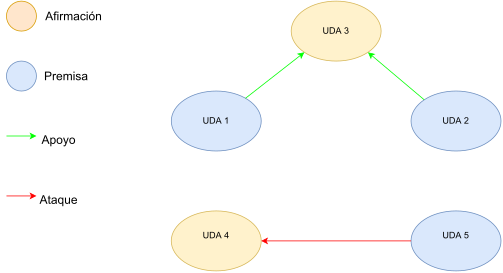
\includegraphics[scale=.7]{Graphics/Estructuras_argumentativas.png}
            % \includesvg[options]{Graphics/Estructuras argumentativas.svg}
        \end{center}
	    \caption{Estructuras Argumentativas.}
	\end{center}
\end{figure}\label{fig:arg_struct}

% TODO 

En el trabajo se desarrolla un modelo cuyo objetivo es la extracción de dichas estructuras argumentativas. 
La extracción de estas componentes constituye una tarea que permite ... TODO seguir esto.

\chapter{Marco te'orico y preliminares}\label{chapter:background}

% Introducción a Deep Learning, Neural Networks: Tipos de aprendizaje, esquema de minimización.
% Explicaciones de los modelos usados: Funciones de activacion, Relu, softmax
% Explicaciones de los modelos usados: Funciones de error, categorical crossentropy
% Explicaciones de los modelos usados: LSTM y Bidireccional, CRF, CNN, ResNet, DenseLayer, GloVe, Attention
% Explicaciones de los modelos usados: Optimizadores Adam, Stocastic Gradient Descent, Diferenciacion automática

En este cap'itulo se introducen conceptos de aprendizaje automático. Temas
como la representación de datos, arquitecturas, evaluación de modelos son tratados en sus secciones.
Se menciona las diferentes investigaciones realizadas en la EA a lo largo de los annos, viendo
los enfoques tomados y la evoluci'on de estos a partir del desarrollo e introducci'on de nuevos m'etodos en el
campo. Por 'ultimo se introduce la proyección de corpus, t'ecnica necesaria para la creación de conjuntos 
de datos necesarios para el entrenamiento de modelos de aprendizaje automático.

\section{Aprendizaje Automático}

Existen varios problemas para los cuales es difícil escribir un programa de forma tradicional que pueda
resolverlo, como decir si en una imagen existe un gato o un perro, o transcribir una grabación. En el caso
de que se escribiera este programa probablemente sería frágil y poco escalable. El aprendizaje automático
(AA) constituye el estudio de técnicas que puedan 
aprender de la experiencia [\cite{d2l}]. Con esto se puede automatizar el proceso de encontrar soluciones a 
dichos problemas, haciendo que sus resultados sean robustos y escalables. En AA existen tres tipos de 
aprendizaje, el aprendizaje no supervisado TODO ESCRIBIR. Otro tipo de aprendizaje es el reforzado el cual 
TODO ESCRIBIR. Finalmente se encuentra el aprendizaje supervisado TODO ESCRIBIR. A este útlimo principalmente 
se refiere la sección.

Los componentes básicos de un problema de aprendizaje supervisado se pueden resumir en los datos de los que 
aprender, el modelo para transformar los datos, una función de pérdida que cuantifica qué tan malo o bueno es el 
modelo y un algoritmo que ajuste los parámetros del modelo para minimizar la pérdida.

Matemáticamente un modelo constituye una función $\hat{y} = f_{\theta}(x)$ a la cual se 
le pasan representaciones de las entradas orginales $x$ y devuelve una salida $\hat{y}$. Esta función $f$ se encuentra
parametrizada por el vector $\theta$ el cual constituyen los parámetros en los que el modelo se basa para realizar sus
cálculos. La función de pérdida se puede definir como $e(y, \hat{y})$. El objetivo final del algoritmo de ajuste 
se define como encontrar $\theta$ tal que (\ref{eq:arg_min_theta}):

\begin{equation}
	\arg \min_{\theta} e(Y, f_{\theta}(X))
\end{equation}\label{eq:arg_min_theta}

Los parámetros $\theta$ eventualmente se van ajustando con algún algoritmo de optimización para que alcance 
un valor óptimo, aunque un mínimo global en la práctica es dificil de conseguir.

Una manera de observar la complejidad de estos modelos sería la cantidad de capas de procesamiento que lo integran.
En los principios se empezaron utilizando modelos de una sola capa\footnote{A estos modelos se les conoce 
como \emph{shallow} o poco profundos} para realizar 
las tareas, más tarde estos modelos fueron ganando en complejidad al superponerle otras dando paso al 
aprendizaje profundo (\textbf{DL} por sus siglas en inglés \emph{Deep Learning}). La superposición se refiere
a la composición de funciones $f_i$ y $f_{i+1}$ de tal forma que la imagen de $f_i$ sea compatible con el dominio de 
$f_{i+1}$ entonces se obtiene $f_{i+2}(x) = f_{i+1}(f_i(x))$, al aplicar este esquema se pueden agregar múltiples
capas y profundizar $f$ tanto como se desee.


\subsection{Representación de datos}

La representación de los datos constituye una parte importante en modelar un problema. Esta 
es la encargada de presentar datos abstractos, como imágenes, párrafos, sonidos, en formas tratables
por los algoritmos. Generalmente se buscan configuraciones que recojan la mayor cantidad de información 
de la entrada relevante al problema.

En PLN la representación suele estar representada a distintos niveles de granulidad.
De menor granulidad a mayor se pueden ir mencionando los documentos, párrafos, oraciones, palabras y
caracteres. De estos elementos es posible representarlo mediante vectores que codifiquen propiedades
objetivas del problema a tratar como características morfológicas o semánticas de estos.

Las características morfológicas son aquellas que describen cómo está formado el elemento a analizar.
Estas pueden ser extraídas con relativa facilidad, entre tales características se encuentran tamaño, 
cantidad, posición de palabras o párrafos, presencia de sufijos, prefijos, acentos u otros marcadores
en el texto. Las características semánticas presentan una mayor dificultad a la hora de ser extraídas.
Para esto se utilizan diferentes modelos que codifican esta información en vectores conocidos como 
\emph{embeddings}. Para esto se existen varios modelos 
como \textbf{word2vec} [TODO ref], \textbf{GloVe} (TODO Poner que signica las siglas y Referencia), \textbf{BERT}
(TODO Poner que signica las siglas y Referencia).
En \textbf{word2vec} modelan ... (TODO continuar), \textbf{GloVe}
sigue el enfoque de ... (TODO continuar). \textbf{BERT} se basa en ... (TODO continuar, poner las variantes RoBERTa, etc).

\subsection{Modelaci'on de problemas}

TODO Empezar con intro
TODO Hablar de problemas de clasificación
TODO Hablar de los modelos seq2seq, Hablar del etiquetado BIO y BIOES, hablar de agregar meta etiquetas a este 
tipo de problemas.


\subsection{Arquitecturas}

En aprendizaje profundo existen una gran cantidad de arquitecturas que se pueden utilizar para formar el modelo 
final.

\subsubsection{Capas densas}

El perceptron consiste es una transformación lineal del vector de datos $\textbf{x}$ con un bias $b$ y 
luego aplicar una transformación no lineal $g$, conocida como función de activación, 
para la obtención del resultado final:

\begin{equation}
	f(\textbf{x}) = g(\textbf{w}\textbf{x} + b)
\end{equation}\label{eq:perceptron}.

El perceptron constituye la unidad básica de las capas densas, ya que estas consisten en la aplicación
de este modelo varias veces sobre la misma entrada $\textbf{x}$ produciendo vectores de la dimensión $k$ 
deseada como salida final. Los parámetros se codifican en la matriz $W$ y sus bias en el vactor $b$:

\begin{equation}
	f(\textbf{x}) = g(\textbf{Wx} + \textbf{b})
\end{equation}\label{eq:dense}.

Para las funciones de activación existen varias elecciones. Una de estas es la función sigmoide. 
Esta devuelve un valor entre 0 y 1, es usada en tareas de regresión logística. 
Se puede interpretar como el nivel de activación de la neurona:

\begin{equation}
	sigm(x) = \frac{1}{1-e^{-x}}
\end{equation}\label{eq:sigmoide}.

\emph{Rectified Linear Unit} (ReLU) es definida como la parte positiva del argumento. Una ventaja que trae esta 
función de activación es su rápido cálculo de su derivada y que previene en parte de los problemas 
de desaparición de gradiente de la sigmoide:

\begin{equation}
	relu(x) = \max(0, x)
\end{equation}\label{eq:relu}.

La función de activación softmax es diferente a las anteriores en el sentido que necesita
el vector salida de la capa para ser computada. Esta función convierte las $q$ salidas
de la en una distribución de probabilidad, por esto es utilizada en tareas de clasificación:

\begin{equation}
	softmax_k(\textbf{x}) = \frac{e^{x_k}}{\sum_{i=1}^q x_i}
\end{equation}\label{eq:softmax}.

\subsubsection{Redes Neuronales Convolucionales}

Las redes neuronales convolucionales (\textbf{CNN} por sus siglas en inglés \emph{Convoutional Neural Networks}) 
son un tipo de redes usadas
principalmente en tratar datos en los que su estructura espacial es relevante, por ejemplo
en datos bidimensionales como imágenes y en unidimensionales como sonido y texto.
Estas redes aplican de una función de kernel sobre los datos, $f * g$ donde $f$ son los
datos, $g$ es el kernel o filtro y $*$ es el operador de convolución. La función $g$ se puede 
aprender en el proceso o también puede ser una función de agrupación predefinida. 
Un ejemplo bidimensional de una función de kernel constituye el siguiente caso:

TODO PONER UNA FOTO DE CONVOLUCION DE KERNEL

En este se observa cómo una nueva representación es computada al correr el kernel por la matriz de datos. Este
corrimiento se puede realizar de diferentes formas, por ejemplo se puede mover de dos en dos en vez de uno en uno, este
parámetro se le conoce como tamaño de paso (\emph{stride} en inglés). Es posible además preservar las dimensiones
iniciales de los datos al aplicarle un aumento de los datos en los bordes de tal forma que el resultado sea de la misma
dimensión, este aumento es generalmente rellenando convenientemente con 0 los espacios.

TODO PONER UNA FOTO DE CONVOLUCION DE KERNEL CON PADDING Y STRIDE DIFERENTE

Existen varias funciones de agrupación usadas. Entre estas se encuentran las de agrupación máxima, de 
agrupación media. Como sus nombres indican, la de agrupación máxima devuelve el valor máximo de los encontrados
en la ventana del kernel, la de media calcula el promedio de estos valores. Estas capas tienen la capacidad de obtener
información resumida sobre los datos.

\subsubsection{Redes Residuales}

Al crear modelos de aprendizaje profundo se tienen un conjunto de parámetros, las posibles combinaciones 
de estos forman un espacio de funciones $F$ al cual pertenencen todas las posibles instancias del modelo.
Agregar nuevas capas aumenta la complejidad de este, pero no hay garantía de que el viejo espacio 
de funciones $F$ sea subconjunto del nuevo espacio $F'$, lo que implica que el nuevo modelo no es necesariamente
estrictamente superior al antiguo. Este problema es la razón de la aparición de las Redes Residuales. 
Una red residual está formada por 
uno o varios bloques residuales, en los que a la salida de cada bloque residual le es sumada la entrada de 
este mediante una conexión residual.
El objetivo de realizar tal operación es que es posible hacer la contribución del bloque 0 obteniendo así
un modelo equivalente a uno sin el bloque, garantizando la condición de subconjunto $F \subset F'$, además 
dicho bloque no pierde poder expresivo dado que en caso de que su aporte sea considerable al resultado final, 
se tendría que aprender solamente la función $f(x) - x$ donde $x$ es la entrada del bloque para mitigar el 
efecto de la conexión residual y $f$ es la función aprendida por el bloque sin la conexión residual.

TODO FOTO DE RESNET. d2l pag 289

\subsubsection{Redes Neuronales Recurrentes}

Las redes neuronales recurrentes (\textbf{RNN} por sus siglas en inglés \emph{Recurrent Neural Networks}) son
un tipo especial de arquitectura especializada en el trabajo con datos secuenciales. Este tipo de arquitecturas
presentan variables en las que se almacenan información pasada que es usada para el computo de la salida. El 
problema se puede modelar mediante probabilidades mediante la estimación de $P(x_t | x_{t-1}, \dots x_{1})$,
donde existen dos variantes principales, se fija un tamaño de ventana en el tiempo $\alpha$ dando como resultado
$P(x_t | x_{t-1}, \dots, x_{t-\alpha})$ a este tipo de modelos se les conoce como autoregresivos. Otra estrategia
consiste en guardar un contexto de observaciones pasadas $h_t$ y con este realizar la estimación $P(x_t | h_t)$,
el contexto se actualiza en cada paso mediante una función $h_t = g(h_{t-1}, x_{t-1})$, a estos se les nombra
modelos autorregresivos latentes. 

Estos modelos presentan problemas de gradientes ya que estas pueden volverse extremadamente grandes o desaparecer.
Para esto se han creado arquitecturas que disminuyen estos problemas. Una de estas arquitecturas es las memorias
de corto largo plazo (\textbf{LSTM} for sus siglas en inglés \emph{Long Short Term Memory}) [\cite{TODO lstm}].
Este modelo guarda un contexto del procesamiento y está constituído por varias compuertas que regulan las 
actualizaciones de los estados internos. \textbf{LSTM} posee dos variables de estado, la memoria $C$ y el estado 
oculto $H$. Entre sus compuertas se encuentran la compuerta de olvido, esta regula cuanto de la memoria permanece
en el proximo paso, la compuerta de entrada ajusta la cantidad de información nueva que estrará, la compuerta 
de salida maneja el calculo del próximo estado oculto.

TODO FOTO DE LSTM d2l pag 357

El método de aprendizaje de las \textbf{RNN} solamente observa los elementos anteriores de la secuencia, aunque existen
tareas en las que observando los elementos posteriores brinda más contexto e información a la tarea sin que interfiera
en el proceso de inferencia. El modelo bidireccional presenta una alternativa para tratar estas tareas, este modelo
consiste en además de hacer la corrida de inicio a final de la secuencia, se realiza un desde al final hasta el  
inicio de esta, estas corridas van generando dos estados ocultos $\overrightarrow{H}_{i}$ y $\overleftarrow{H}_{i}$
que luego son mezclados para obtener el contexto final $H_i$.

TODO FOTO DE BIDIRECTIONAL LSTM d2l pag 367

\subsubsection{Atención}

% Definicion, qué hace, uso en secuencias
La atención es una técnica en la cual se hace una selección ponderada de atributos en un contexto específico. 
Este mecanismo presenta dos partes, una consulta $q$ y una collección de pares llave-valor $(k_i, v_i)$, la 
consulta representa el contexto en donde se quiere aplicar la atención y las llaves $k_i$ son elementos que 
relacionan la consulta a los valores $v_i$. El proceso de calcular el resultado consiste en primero calcular 
el vector compatibilidad $e$ entre las llaves y la consulta mediante la función $f$, este vector es luego 
modificado por una función $g$ que distribuye los valores obteniendo el vector atención $a$, finalmente 
este vector es utilizado para calcular el resultado final al aplicarle la función $o = z(a, V)$.

\begin{equation}
	e = f(q, K)
\end{equation}
\begin{equation}
	a = g(e)
\end{equation}
\begin{equation}
	o = z(a, V)
\end{equation}

En dependencia de cómo se seleccionen las funciones $f$, $g$ y $z$ se pueden obtener distintos tipos de atención.
Una configuración simple consiste en ser $f$ definida como el producto punto de la consulta con la llave,
$g$ softmax y $z$ la suma ponderada de $v_i$ con los valores de atención. 

\subsubsection{Campo Aleatorio Condicional}

% Definicion de CRF, qué modela, Ventajas de CRF en secuencias, mirar relacion con Hidden Markov Models

El campo aleatorio condicional (\textbf{CRF} por sus siglas en inglés \emph{Conditional Random Field}) es un 
tipo de modelo gráfico probabilístico con el objetivo de modelar eficientemente el trabajo con secuencias 
modelando conjuntamente la probabilidad de las etiquetas de las secuencias dada sus observaciones [\cite{lafferty2001conditional}].
En trabajos de secuencias la forma más simple que toma el grafo consiste en una cadena de las variables representando
las etiquetas de las secuencias $Y$ conectadas de la forma $(Y_i, Y_{i+1})$ y las variables observadas $X$ conectadas
a las variables $Y$ [\cite{wallach2004conditional}].

El objetivo de \textbf{CRF} es calcular la secuencia $Y^*$ tal que:

\begin{equation}
	Y^* = \arg \max_Y P(Y | X)
\end{equation}\label{eq:crf}.

En este se observa que devuelve la secuencia más probable dado las variables observadas o atributos $X$,
por lo que esta capa es usada al final para problemas de clasificación de secuencias.

\subsection{Evaluación del modelo}

En AA los modelos necesitan maneras de expresar qué tan buenos son 
en las tareas encomendadas. Para esto se crean funciones que evalúan los resultados obtenidos
por dichos modelos, estas funciones se les da el nombre de métricas. Existen diferentes tipos de
métricas para tratar con diferentes tipos de problemas. En aprendizaje supervisado una métrica se
define como una función $m_s(Y, \hat{Y})$ donde $Y$ son las predicciones verdaderas y $\hat{Y}$ son las predicciones
hechas por el modelo. En algoritmos de aprendizaje no supervisado como K-Means, K-NN son usadas funciones $m_{ns}(\hat{Y})$
donde $\hat{Y}$ son las predicciones finales. En comparación con su versión supervisada estas funciones no tiene acceso
a las predicciones verdaderas del problema.

\subsubsection{Clasificación}

En problemas de clasificación son empleadas medidas que toman en cuenta la naturaleza discreta de su conjunto im'agen.
Medidas como precisión, recobrado, certeza (\emph{accuracy} en inglés) y F1 son utilizadas principalmente en la 
evaluación de los resultados, mientras que como función de error se usa entropía cruzada comúnmente 
(\emph{cross entropy} en inglés) [\cite{grandini2020metrics}].

La matriz de confusión es una via de representar los resultados de dos clasificadores. Esta matriz en $M_{ij}$ 
indica la cantidad de elementos que clasificó como clase $i$ el primer clasificador y
como clase $j$ el segundo clasificador. En su uso práctico
un clasificador son las etiquetas verdaderas mientras que el otro es el clasificador que se está evaluando. 
En problemas de la clasificación binaria, donde se busca saber si existe pertenencia o no de un elemento a una clase,
se pueden observar los siguientes casos.

\begin{itemize}
	\item Verdaderos Positivos (VP): Elementos clasificados correctamente que pertenecen a la clase.
	\item Verdaderos Negativos (VN): Elementos clasificados correctamente que no pertenecen a la clase.
	\item Falsos Positivos (FP): Elementos clasificados incorrectamente que pertenecen a la clase.
	\item Falsos Negativos (FN): Elementos clasificados incorrectamente que no pertenecen a la clase.
\end{itemize}

TODO FOTO DE MATRIZ DE CONFUSION BINARIA

La precisión es la medida que indica la probabilidad de que la clasificación de una clase sea correcta. Esto 
se puede observar como la proporción de los elementos correctamente clasificados sobre el total de 
elementos clasificados:

\begin{equation}
	prec_i = \frac{VP}{VP + FP}
\end{equation}.

En problemas de clasificación múltiple surge la versión macro de esta medida calculada como la media de todas
las precisiones de las clases existentes:

\begin{equation}
	prec_{macro} = \sum^K_{i=1} \frac{prec_i}{K}
\end{equation}.

El recobrado es la medida que indica la probabilidad de que se clasifique correctamente un elemento de la clase
del total existente. Esto se puede observar como la proporción de los elementos correctamente clasificados sobre el 
total de elementos que pertenecen a la clase:

\begin{equation}
	rec_i = \frac{VP}{VP + FN}
\end{equation}.

En problemas de clasificación múltiple surge la versión macro de esta medida calculada como la media de todos
los recobrados de las clases existentes:

\begin{equation}
	rec_{macro} = \sum^K_{i=1} \frac{rec_i}{K}
\end{equation}.

La medida F1 es la media armónica de la precisión y el recobrado. En esta la contribución de la precisión y el
recobrado al resultado final es el mismo, aunque es posible buscar variaciones de acuerdo a al problema a tratar:

\begin{equation}
	f1_i = 2 (\frac{prec_i · rec_i}{prec_i + rec_i})
\end{equation}.

En problemas de clasificación múltiple surge la versión macro de esta medida calculada la propia medida F1 pero
utilizando la precisión y recobrado macro del problema:

\begin{equation}
	f1_{macro} = 2 (\frac{prec_{macro} · rec_{macro}}{prec_{macro} + rec_{macro}})
\end{equation}.

Las m'etricas anteriores est'an acotadas por los valores 0 y 1 donde 1 representa la mejor evaluación y 0 la 
peor.

La entropía cruzada se encarga de evaluar qué tan diferentes son dos funciones de distribución $p$ y $q$, su 
resultado es un n'umero no negativo que a medida que sean m'as pequeños los valores indican mayor similitud. 
En su versión discreta se formula:

\begin{equation}
	H(p, q) = - \sum_{x \in D} p(x) \log q(x)
\end{equation}

\subsubsection{Curvas de aprendizaje}

Es necesario además de evaluar el resultado final del modelo, evaluar el proceso de entrenamiento. En esta etapa 
se pueden diagnosticar varias deficiencias en este proceso. Para un correcto diagnóstico se divide el conjunto de 
datos en tres partes:

\begin{itemize}
	\item \textbf{entrenamiento}: Utilizada para el entrenamiento del modelo.
	\item \textbf{validación}: Utilizada para evaluar el desempeño del modelo en entrenamiento.
	\item \textbf{prueba}: Utilizada para evaluar el resultado final.
\end{itemize}

Las curvas de aprendizaje constituye la principal herramienta para evaluar el proceso de aprendizaje.
Estas están formadas por las mediciones de métricas a lo largo del entrenamiento calculadas a partir de 
los conjuntos de validación y entrenamiento. La linea correspondiente al conjunto de entrenamiento cuantifica 
el aprendizaje del modelo o también el error de entrenamiento y la correspondiente a la de validación cuantifica 
la generalización o el error de generalización. Existen tres comportamientos escenciales:

\begin{itemize}
	\item Bajo ajuste (\emph{underfitting} en inglés).
	\item Sobreajuste (\emph{overfitting} en inglés).
	\item Buen ajuste.
\end{itemize}

El bajo ajuste ocurre cuando el modelo no es capaz de aprender del conjunto de datos o cuando este aún puede aprender 
más. Las curvas de aprendizaje en estos casos se caracterizan por ser una linea plana o valores ruidosos con alta pérdida.

TODO FOTO de LO DICHO ANTERIOR. Guiarse por el libro [brownlee2018better]

Entre las formas más sencillas de combatir el bajo ajuste de los modelos consiste en complejizar el modelo, al añadir
capas o aumentar las dimensiones se este aumenta la expresividad de este y por lo tanto su ajuste. Si este método 
no funciona es posible considerar un cambio de arquitectura hacia una que pueda extraer más información de la 
estructura de los datos. 

El sobreajuste es el fenómeno en el que el modelo se aprende los datos de entrenamiento extremadamente bien, incluso
el ruido en estos datos, esto trae consigo que falla en generalizar el problema para nuevas entradas. Las curvas 
características de este fenómeno presentan una divergencia en los errores de entrenamiento y validación a medida
que se entrena el modelo, mientras que la de entrenamiento mejora la de validación tiende a empeorar. 

TODO FOTO de OVERFITTING. Guiarse por el libro [brownlee2018better]

Existen varios métodos para combatir el sobreajuste, uno sencillo es simplificar el modelo quitándole capas 
o disminuyendo sus dimensiones. Además de esto existen regularizaciones que se pueden aplicar para evitar que 
las capas dependan exclusivamente de pocos atributos, entre esta familia los más usados son la regularización
L1 y L2 las cuales se definen como la suma del valor absoluto de los atributos y la suma del cuadrado de sus 
atributos respectivamente. Otra medida para prevenir el sobreajuste es el agrego de capas de abandono 
(\emph{dropout} en inglés), estas capas desactivan neuronas de la arquitectura y obligando a 
estas a ser robustas y depender del comportamiento de la población, en lugar de la actividad de otras unidades 
específicas [\cite{baldi2013dropout}]. La terminación temprana (\emph{early stopping} en inglés) del entrenamiento
se utiliza para parar este en el momento en que el error de generalización comienza a subir, impidiendo así que 
se sobreentrene el modelo.

Finalmente un buen ajuste es el resultado que se alcanza cuando tanto la curva de validación como de entrenamiento
presentan valores pequeños y similares, consecuentes con una correcto aprendizaje y generalización.

TODO FOTO de Good Fit. Guiarse por el libro [brownlee2018better]

Otro problema observable a partir del análisis de las curvas de aprendizaje constituye la detección de conjuntos
de datos no representativos. Un conjunto de datos no representativo es uno que puede no 
capturar las características estadísticas relativas a otro conjunto de datos extraído del mismo dominio.
Esto puede pasar que los conjuntos de entrenamiento o de validación. En caso del conjunto de entrenamiento
se puede identificar si la pérdida en el conjunto de entrnamiento conlleva a una ganancia en el conjunto de 
validación y viceversa quedando al final con una separación entre ambos valores. En el caso del conjunto de 
validación se presenta como una curva ruidosa, también se puede dar el caso de que el conjunto  de validación
sea más fácil de predecir que el de entrenamiento, en este caso se observa como la curva de validación permanece
siempre por debajo de la de entrenamiento.

TODO FOTO de Unrepresentative Train Data, Unrepresentative Dev Data (Noise, Easier than train). Guiarse por el libro [brownlee2018better]

Para combatir estos problemas se puede aumentar la cantidad de elementos en los conjuntos de entrenamiento o 
validación en dependencia de donde ocurra.

\subsection{Aumento de datos}

El aumento de datos consiste en acciones para aumentar la diversidad de un conjunto de datos sin recolectar
nuevos datos explícitamente [\cite{feng2021data}]. En datos continuos, como imágenes o valores numéricos el 
aumento de datos puede ser realizado al añadirle perturbaciones a entradas existentes, en caso de las imágenes 
técnicas como el volteado (\emph{flipping}) o recortado (\emph{cropping}) son usadas. Los textos son un tipo 
de datos discreto y por lo tanto las técnicas anteriores no pueden ser aplicadas directamente. Para PLN
se han estudiado diversas técnicas para el aumento de datos, una de estas consiste en el cambio del árbol de 
dependencia de la oración mediante operaciones de intercambio y borrado de nodos [TODO \cite{}], también se han utilizado 
gaceteras para el intercambio de palabras por sinónimos [TODO \cite{}], la traducción de textos hacia un lenguaje y luego 
de vuelta al lenguaje origen es otro ejemplo o \emph{backtranslation} en inglés. 

\subsection{Aprendizaje Conjunto}

El aprendizaje conjunto (\emph{ensemble learning} en inglés) constituyen técnicas encaminadas al aprovechamiento
de soluciones encontradas por diferentes modelos combinándolas y mejorándolas para encontrar una mejor solución 
al problema. Estos métodos son efectivos en la reducción de la varianza y el bias de los resultados obteniendo así
mejores resultados [\cite{dietterich2002ensemble}] 

Las manera TODO

\subsection{Métodos de optimización}

% Optimización, encontrar la solucion exacta es un problema dificil, se usan metodos para buscar soluciones aproximadas.
% Descenso por gradiente Algoritmo general, Optimizadores (Adams, Stocastic Gradient Descent, Exponential Decay)

El objetivo de AA es encontrar los extremos de una función de costo, este proceso es una tarea 
desafiante ya que la gran mayoría de estas funciones no son convexas y por lo tanto no existe un algoritmo
que asegure la convergencia hacia un extremo global. Para resolver este problema exiten múltiples heurísticas,
la más usasda es el descenso por gradiente, este algoritmo contiene múltiples variaciones. La idea básica consiste 
en el cálculo del vector gradiente de la función de error $e$ con respecto a los parámetros del modelo $x$ y una vez se 
tiene dicho vector se evalua en la asignación actual de los parámetros $x_i$ y se realiza un corrimiento de este punto 
en contra del gradiente para disminuir el error.

\begin{equation}
	x_{i+1} = x_i - \alpha \nabla f(x_i)
\end{equation}\label{eq:gradien_descent}

En la ecuación anterior $\alpha$ se le conoce como tasa de aprendizaje (\emph{learning rate} en inglés),
este valor cuantifica cuánto se toma del vector del gradiente para actualizar los parámetros, esto 
se puede ver como el aprendizaje del modelo.

Variantes de este algoritmo eficientes para el proceso de entrenamiento de modelos de AA han sido 
creadas. Entre las técnicas utilizadas se encuentran Descenso por Gradiente Estocástico (\textbf{SGD} por sus siglas 
en inglés \emph{Stochastic Gradient Descent}) [TODO \cite{}], tasa de aprendizaje dinámica con sus diferentes
variantes (exponencial, polinómica) [TODO \cite{}], RMSProp [TODO \cite{}] y Adam [TODO \cite{}]. 

\section{Extracción de Argumentos}

Varias investigaciones y propuestas han salido para dar respuesta a los problemas asociados a EA, mostrando
una variedad en enfoques y métodos.

En [\cite{palau2009argumentation}] se propone
el uso de modelos estadísticos como \emph{Naive Bayes} (\textbf{NB}) y \emph{Support Vector Machine} (\textbf{SVM}) 
para la clasificación de 
oraciones en argumentativas o no y en su rol argumentativo en caso de que sea argumentativa, en este
caso se asume que las componentes argumentativas son oraciones completas. Para la predicción de relaciones
se usa un enfoque basados en reglas con la creación de una Gramática Libre de Contexto. Las representaciones
de las oraciones se ven dadas por atributos creados a mano, dado el conocimiento experto sobre la argumentación
en el tema tratado, elementos como adverbios, verbos, signos de puntuación, palabras clave, estadísticas del texto
(Tamaño de oración, distancia media de palabras) son usados para la extracción y clasificación de las UDA, además
se usan también como base en la creación de las relgas de la gramática para la extracción de relaciones.

[\cite{goudas2015argument}] al igual que [\cite{palau2009argumentation}] clasifica las oraciones como
argumentativas o no mediante el uso de diferentes clasificadores como \textbf{NB}, \emph{Random Forest}, Regresión
Logística y \textbf{SVM}. En este trabajo se aumenta la grandularidad de la segmentación al permitir
la extracción de los segmentos que contienen la carga argumentativa de dentro de las oraciones previamente clasificadas
como tal, esto se realiza mediante la extracción de etiquetas BIO de las oraciones con el uso de un 
\textbf{CRF}. La predicción de las relaciones es modelado como un problema de clasificación
usando \textbf{SVM} para clasificar pares de UDA en relacionados o no. Atributos creados a mano 
son usados en la extracción de UDA entre estos están posición de la oración en el texto, cantidad de verbos, comas, adverbios,
palabras, entidades en la oración, también se emplean gaceteras que guardan entidades relacionadas con el dominio 
específico y palabras clave indicadoras de frases argumentativas. 

[\cite{stab2017parsing}] propone un mecanismo de segmentación basado en \textbf{CRF}. La clasificación
y predicción de relaciones es modelado conjuntamente como con dos clasificadores \textbf{SVM} y un problema
de Optimización Lineal Entero que encuentra la mejor estructura y asegurar una disposición arborea. En la segmentación
de las UDA se extraen por cada token su posición en el texto, si precede o sucede a un signo de puntuación, su parte de
la oración, la probabilidad de que sea el comienzo de una UDA dado sus tokens anteriores, entre otros. Para la extracción
y clasificación de relaciones se proponen otros conjuntos de atributos como la cantidad de sustantivos comunes entre
las componentes fuente y el objetivo, la presencia de indicadores argumentativos, representaciones vectoriales de tokens.

En [\cite{eger2017neural}] se enfocaron en presentar el problema de EA como uno \emph{end-to-end}. 
Para esto presentaron varias propuestas, entre ellas se encontraba
modelar el problema como un uno de secuencia a secuencia, usando \textbf{RNN} como 
\textbf{LSTM} en versiones bidireccionales capturando información desde ambos lados de la secuencia,
para la representación de las palabras se extrajo información morfológica de las palabras mediante Redes Neuronales Convolucionales,
al final realizan la clasificación de la secuencia con un \textbf{CRF}. 
Realizaron experimentos al modelar el problema como uno de \emph{Dependency Parsing} en [\cite{kiperwasser2016simple}]. Este problema
consiste en construir un árbol de dependencia que codifique las estructuras argumentativas, en este problema 
se tiene que decidir entre varias opciones (\emph{shift}, \emph{reduce}) en dependencia del contenido de la pila y en el buffer.
El problema fue modelado también como un problema de reconocimiento de entidades nombradas, en donde las entidades son las UDA.

[\cite{galassi2018argumentative}] propone el uso de redes residuales y en combinación con mecanismos de atención
para la creación de un modelo el cual, conjuntamente, clasifica el tipo de UDA y la relación existentes entre estas.
Este trabajo define el concepto de distancia argumentativa, añadiéndolo como feature y asume que las UDA ya fueron 
extraídas. En este caso además de la distancia argumentativa las secuencias son representadas por sus representaciones
vectoriales de \textbf{GloVe}. Este trabajo asume la previa extracción de las UDAs.

En [\cite{dykes2020reconstructing}] se propone métodos basados en reglas para la extracción de argumentos sobre
textos en Twitter, estos métodos se centran en la confección de reglas basadas en anotaciones lingüísticas como
partes de la oración, lemas de palabras. La recuperación está basada en los esquemas argumentativos comunes presentes
en los textos. Este método apunta a una mayor precisión prescindiendo de recobrado. Dada las reglas creadas y el tipo
de datos con que se trabaja, cadenas de texto pequeñas, estos algoritmos tienden a tener una alta precisión aunque 
bajo recobrado, esto en conjuntos de datos grandes no es un gran problema, pero en conjuntos de menor tamaño o estructura 
más compleja pierden efectividad.

En resumen se contempan disímiles enfoques al problema de EA desde una perspectiva enmarcada en modelos 
simbólicos, estadísticos y neuronales en versiones tanto secuenciales como \emph{end-to-end}. 
Cada uno de estos modelos presentan sus ventajas y desventajas a la hora de contruirlos, 
extenderlos y comprender su funcionamiento. En modelos simbólicos se presenta una alta
precisión en dominios específicos debido a que estos se construyen teniendo en cuenta reglas específicas a un
contexto dado. Estos modelos son poco escalables y difíciles de mantener ya que son sus reglas son construídas
a mano y dicho proceso requiere de conocimiento experto y tiempo. Modelos estadísticos son
característicos de usar conjuntos de atributos creados a mano, dichos atributos son difíciles
de encontrar, calcular y pueden no poseer relevancia en otros contextos diferentes a los que fueron creados. 
Además la necesidad de conocimiento experto es necesaria para su confección. Los modelos neuronales poseen
un mayor poder de adaptabilidad, en estos la entrada es codificada en una representación que es aprendida por
el mismo algoritmo, permitiendo seguir viable para distintos esquemas argumentativos. Los modelos simbólicos y 
estadísticos poseen la ventaja de poder explicar el porqué de los resultados devueltos cosa que se vuelve casi
imposible en modelos neuronales.

Dado que la EA es un proceso en el cual se necesita pasar por varias tareas, estas deben de ser completadas
de alguna forma. Una manera de completarlas es hacerla una a la vez, independiente una de otra y pasándole
la salida de etapas anteriores a las etapas siguientes. Esta manera secuencial de realizar las 
tareas es bastante simple y ayuda a la creación de modelos simples y con tareas bien definidas, aunque trae consigo 
la propagación de los errores a través del proceso y el no aprevechamiento de las interrelaciones entre variables 
computadas de procesos anteriores. Modelos \emph{end-to-end} en cambio poseen la habilidad de modelar el problema 
desde su inicio hasta su final de manera conjunta, mediante \emph{Multi-Task Learning} (\textbf{MTL}) se modelan
las tareas de manera conjunta creando modelos complejos aunque con una propagación de error menor.

\section{Proyección de corpus}

La EA no es un campo de PLN que presenta una gran cantidad de datos anotados con los cuales se pueda realizar 
un entrenamiento, además de esto la gran mayoría de corpus existentes se encuentran en lenguajes como inglés o alemán,
haciendo difícil el desarrollo de esta rama en otros lenguajes.
La escasez de estos datos es en gran parte debida al elevado costo monetario, de tiempo y de recursos humanos que se utiliza
en su creación. En orden de poder desarrollar la EA en otros lenguajes, como el español, se han investigado diferentes vertientes
para la construcción de conjuntos de datos en estos lenguajes de pocos recursos a partir de los conjuntos de datos ya 
existentes.

La proyección de etiquetas consiste en un algoritmo en donde se 
transfieren las etiquetas de un corpus anotado a nivel de tokens en un lenguaje origen hacia su traducción en un 
lenguaje objetivo. Transferencia directa se refiere a (TODO completar)
En [\cite{eger2018cross}] se muestra que la proyección constituye una mejor alternativa sobre la transferencia
directa y presentan un algoritmo para realizar la proyección de las etiquetas dadas las alineaciones de palabras.
El proceso se divide en varias partes:

\begin{enumerate}
	\item Traducción de oraciones.
	\item Alineación de palabras.
	\item Proyección de etiquetas.
\end{enumerate}

\subsection{Traducción de oraciones}

La Traducción Automática consiste en el proceso de usar inteligencia artificial para
traducir texto de un lenguaje fuente a un lenguaje objetivo sin la intervención humana.
En la actualidad este campo ha dado un gran paso pasando de modelos estadísticos a modelos
neuronales llevando a tener traducciones de una alta calidad sin variar significativamente de la humana, 
condición necesaria para una buena proyección [\cite{eger2018cross}].

Por lo anterior es posible la traducción de corpus hacia otros lenguajes mediante las
herramientas existentes obteniendo una buena representación final, la cual se puede usar en la creación de
oraciones alineadas, primer paso para la proyección de etiquetas.

\subsection{Alineación de palabras}

La alineación de palabras consiste en encontrar las palabras generadas en el lenguaje objetivo por las 
palabras en el lenguaje fuente.
Este problema es atacado en los modelos IBM, modelos estadísticos de traducción automática que usan estos 
índices para obtener más información. Estos modelos son principalmente Bayesianos y han sido la base de
otras herramientas como FastAlign [\cite{dyer2013fastalign}] que incorpora una reducción sustancial del
tiempo de cómputo y además de una mejora al modelo, EFMARAL [\cite{ostling2016efficient}] que usa
Cadenas de Markov Monte Carlo. Modelos más recientes se han enfocado en explotar las representaciones
vectoriales de palabras y el uso de métodos de atención para la extracción de las
alineaciones [\cite{dou2021word}].

FOTO de EJEMPLO de ALINEACION

\subsection{Proyección de etiquetas}

La proyección de etiquetas consiste en transportar las etiquetas de las palabras en la secuencia origen
hacia las palabras de la secuencia destino tomando como datos las alineaciones entre estas. En [\cite{yarowsky2001inducing}]
se trata el problema de proyección de frases nominales, estas frases tienen como característica que son resistentes
a ser divididas en caso de ser traducidas, dicha propiedad se cumple para las UDA también, que aunque evidencian 
cambios en el orden de las palabras, mantienen la misma ventana. La proyección de UDA son más simples en el caso
que solamente se tiene en cuenta la ventana y las etiquetas en estas son constantes, no pasa con la proyección en
frases nominales las cuales pueden cambiar dentro de una ventana, por lo que algoritmos más simples existen
para esta tarea [\cite{eger2018cross}].

\chapter{Propuesta}\label{chapter:proposal}

El modelo propuesto se divide en dos secciones. En la primera sección se realiza la segmentación y clasificación de 
las UDAs como tareas conjuntas. En la segunda sección se predicen los enlaces y sus clasificaciones, tomando
como tareas auxiliares la clasificación de las UDAs. Dada la heterogeniedad de las conjuntos de datos disponibles 
en EA los modelos poseen un mínimo de atributos, esto permite que el modelo por sí solo aprenda 
la mejor representación para el esquema de anotación con que se entrene.

\section{Segmentación y clasificacón de UDAs}

Esta primera parte se modela como un problema secuencia a secuencia cuyo objetivo es asignar a los tokens 
extraídos del documento entrada una etiqueta BIOES para segmentar las UDAs. Para la clasificación del tipo 
de UDA al conjunto de etiquetas BIES se le añadieron las clasificaciones que presentan el corpus entrenante.
En el siguiente ejemplo se presentan las meta-etiquetas
$A$ como Argumento y $P$ como premisa.

\begin{adjustwidth}{25pt}{25pt}
    En$_O$ primer$_O$ lugar$_O$ ,$_O$ [\emph{el$_{B-A}$ correo$_{I-A}$ electrónico$_{I-A}$ puede$_{I-A}$ 
    contar$_{I-A}$ como$_{I-A}$ uno$_{I-A}$ de$_{I-A}$ los$_{I-A}$ resultados$_{I-A}$
    más$_{I-A}$ beneficiosos$_{I-A}$ de$_{I-A}$ la$_{I-A}$ tecnología$_{I-A}$ moderna$_{E-A}$}] .$_{O}$ 
    [\emph{Años$_{B-P}$ atrás$_{I-P}$ ,$_{I-P}$ las$_{I-P}$ personas$_{I-P}$ pagaban$_{I-P}$ gran$_{I-P}$ cantidad$_{I-P}$ 
    de$_{I-P}$ dinero$_{I-P}$ para$_{I-P}$ enviar$_{I-P}$ sus$_{I-P}$ cartas$_{I-P}$ y$_{I-P}$ sus$_{I-P}$ 
    pagos$_{I-P}$ estaban$_{I-P}$ sujetos$_{I-P}$ al$_{I-P}$ peso$_{I-P}$ de$_{I-P}$ sus$_{I-P}$ 
    cartas$_{I-P}$ o$_{I-P}$ paquetes$_{I-P}$ y$_{I-P}$ muchos$_{I-P}$ accidentes$_{I-P}$ podrían$_{I-P}$
    causar$_{I-P}$ problemas$_{I-P}$ que$_{I-P}$ causarían$_{I-P}$ que$_{I-P}$ el$_{I-P}$ correo$_{I-P}$ 
    no$_{I-P}$ fuera$_{I-P}$ enviado$_{E-P}$}] .$_{O}$
\end{adjustwidth}

\subsection{Modelo}

TODO Cambiar los nombres de las dimensiones a un solo caracter, vincular los nombres con la foto.

Sea $D$ un documento entrada, este es separado en una secuencia de $n$ tokens $D_i$ donde $n$ es la mayor longitud encontrada
en los documentos del conjunto de datos (si la cantidad de tokens es menor que $n$ entonces $D_i$ es completado con un token especial de enmascarado). 
A cada token se le es asignado
su representación vectorial \textbf{GloVe} de dimensión $g=300$ dando como resultado $G_{ij} \in \mathbb{R}^{n \times g}$.
Esta representación inicial presenta información semántica de las palabras además que conserva las relaciones 
espaciales entre ellas. 

Para la representación de información morfológica de la palabra se construyen dos
codificadores que procesan los caracteres de cada token y devuelven una representación vectorial de estos.
A cada caracter se le es asignado un vector que será entrenado convirtiendo un token en un vector de dimensión
$q \times c$ donde $q$ es el tamaño máximo de palabra en el conjunto de datos y $c$ es la dimensión del vector
asignado a cada caracter.
Uno de estos modelos está basado en \textbf{CNN}, este modelo entrena una representación de caracteres de dimensión
$cd=50$ representando un token como un vector de dimensión $q \times cd$. Se conforma por una capa de convolución unidimensional
con $f=30$ filtros y un kernel de tamaño $k=3$ seguida por un \textbf{Max Pool Layer} que convierte la secuencia en un vector
de dimensión $1 \times f$ que luego este vector es concatenado a la representación del token a que pertenece.
Otro modelo utilizado para calcular una representación morfológica se encuentra basado en \textbf{RNN}. Se usó
un modelo \textbf{LSTM} bidireccional con dimensión $l=25$ para calcular la representación del token, para las dimensiones de los caracteres se
utilizan vectores de tamaño $l$, el resultado final constituye la concatenación de la corrida hacia adelante y
hacia atrás formando una representación de dimensión $1 \times 2 \cdot l$ del token. Este vector es concatenado a la representación
del token correspondiente.

Otro atributo usado en la representación de los tokens constituyen las etiquetas de Partes de la Oración de estos.
El conjunto de etiquetas elegido es un conjunto universal [\cite{petrov2011universal}] aplicable a cualquier idioma.
De estas etiquetas se les extraen la codificación \emph{one-hot} y esta es transformada por una capa densa con $p=5$ neuronas
y función de activación \emph{ReLU}, el resultado es concatenado a la representación del token correspondiente.

Del proceso de vectorización sale un vector con dimensión $n \times t$ donde $t$ es la dimensión final de la representación
de los tokens. Este vector es modificado por una capa \textbf{LSTM} bidireccional de dimensión $m=200$, a esta salida se le 
añade una conexión residual al ajustarle la dimensión con una capa densa. Luego la secuencia es procesada por una 
capa densa de dimensión $k=100$ con activación \emph{ReLU} produciendo una representación final de dimensión 
$q \times k$. Finalmente se utiliza una capa \textbf{CRF}
para la clasificación final de la secuencia en las etiquetas finales. El resultado final constituye un vector
de dimensión $q$ que representa las clasificaciones inferidas por el modelo.

Para prevenir el sobre ajuste se agregaron capas de normalización y de \emph{dropout} entre cada proceso y se usaron regularizaciones
L2 y \emph{dropout} en las capas densas y \textbf{LSTM}, el valor asignado al dropout fue de $0.5$. 
Para prevenir el sobre entrenamiento se aplicó una 
terminación temprana de este cuando no se enontraba una mejora de la función de pérdida en el conjunto de validación,
el criterio de parada fue la no mejora de la función de pérdida en el conjunto de validación por más de 10 épocas.
Como optimizador se utilizó Adam con una tasa de aprendizaje de $0.001$.

\subsection{Posprocesamiento}

La salida del modelo constituye una secuencia de etiquetas en formato BIOES. La secuencia devuelta puede que contenga
errores en la estructura BIOES, por ejemplo, secuencias no terminandas en E, segmentos continuos con más de una meta-etiqueta,
entre otros.
Para la corrección de la estructura se propone el siguiente algoritmo, el cual se divide en dos partes. La primera
parte consiste en arreglar la estructura BIOES, para esto se mantiene una ventana de tamaño
3 sobre la secuencia y asume que la parte anterior a la posición de la ventana no presenta errores, al encontrar una
ventana inválida se necesita observar la siguiente ventana para poder decidir cómo se arregla el error ya que se
podría dar el caso de OOI OIO, en donde solamente viendo la primera ventana no se podría saber si el cambio 
correcto corresponde a sustituir I por B o por S. Una vez observado las dos ventanas se procede a realizar el 
arreglo correspondiente. En casos donde sea ambigua la manera de arreglar la ventana, IIO (La I o la O pueden ser 
sustituidas por una E) por ejemplo se utiliza una función que recibe un segmento y devuelve la gravedad del error,
el error con mayor gravedad será arreglado, en caso de ser iguales se arreglará la etiqueta más a la izquierda.
Este procedimiento devuelve una secuencia BIOES correctamente anotada, debido a que a partir de una secuencia sin 
errores en cada paso se va arreglando la ventana y una vez esta llega al final arregló todos los elementos de la secuencia.
Una vez se tiene la secuencia tiene la estructura BIOES correctamente anotada el problema
consiste en arreglar las meta-etiquetas, ya que una misma secuencia BIOES pudo haber sido anotada con diferentes
tipos, en este caso se toma la etiqueta más representativa de la secuencia.

\begin{figure}[p]
	\begin{center}
		\begin{center}
			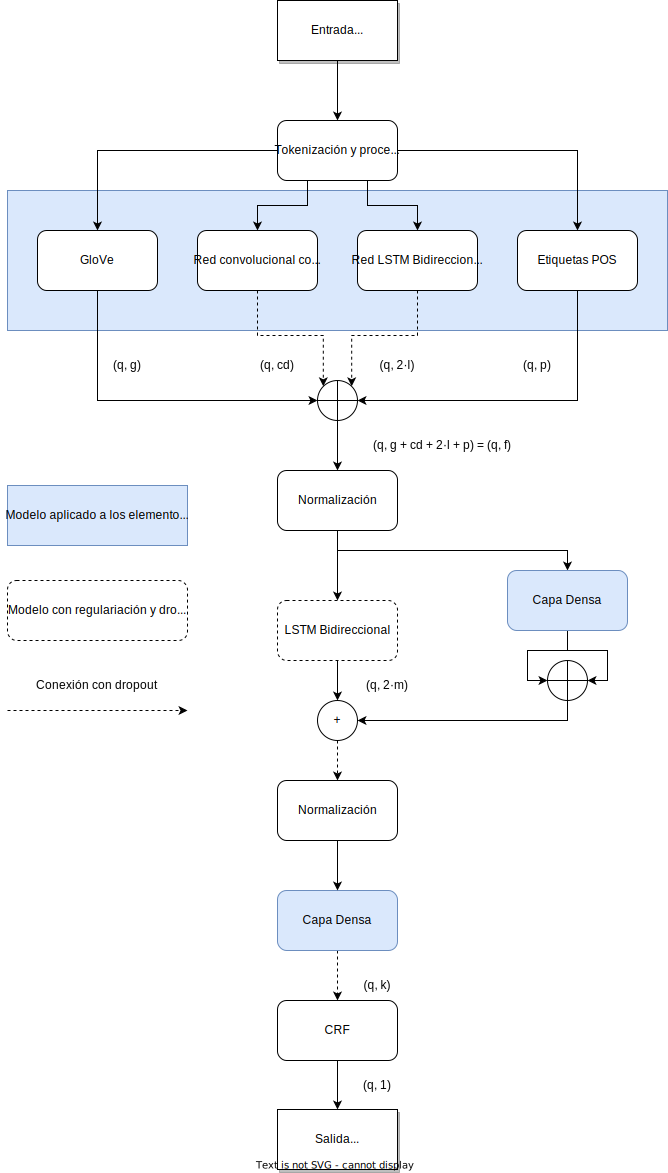
\includegraphics[scale=.5]{Graphics/Modelo_Segmenter_UDA.png}
        \end{center}
	    \caption{Segmentador UDAs.}\label{fig:segmenter_model}
	\end{center}
\end{figure}

\newpage

\section{Predicción de enlaces}

Este modelo consiste en dados dos pares de UDA previamente extraídas, 
extraer y clasificar la relación entre ellas, como tarea auxiliar se realiza además la clasificación 
de las UDAs. Su salida consiste en una tupla conteniendo las clases de relación, tipo de UDA fuente y 
tipo de UDA objetivo respectivamente $(r \in R, s \in U, t \in U)$ donde $R$ y $U$ son los conjuntos de 
posibles tipos de relaciones más una clasificación que representa que no están relacionadas y los tipos de UDAs 
del corpus con que se entrena.

\subsection{Modelo}

Sea dos UDAs, $S$ y $T$, una representa la fuente de la relación, mientras que la otra representa
el objetivo. Estas secuencias son tokenizadas y se les asigna la representación \textbf{GloVe} de cada palabra, obteniendo
dos vectores de dimensión $u \times g$, donde $u$ es el tamaño máximo de UDAs en el conjunto de entrenamiento
y $g=300$ es la dimensión del \emph{embedding}.
Estos vectores son modificados por una red densa compuesta por $ca = 4$ capas con activación \textbf{relu}. 
Al finalizar este procesamiento se añade una conexión residual
a la salida. El próximo paso consiste en aplicar una capa densa de dimensión $di=50$ y luego un \emph{average pooling}
de tamaño $dp$, obteniendo vectores de dimensión $\frac{q}{dp} \times di$. 
Estos vectores son modificados por un \textbf{LSTM} bidireccional con $lm=50$ unidades. Un módulo de atención es aplicado 
sobre los vectores fuentes, 
en este actúan como consultas el promedio de los vectores objetivo y como llaves y valores los vectores fuentes,
el procedimiento simétrico es realizado para los vectores objetivos.
La salida de los procesamientos son concatenados con la distancia argumentativa obteniendo una representación 
conjunta de la relación a analizar. Esta representación conjunta es modificada por una red residual obteniendo
una representación final de dimensión $ff$ y luego sometida a los clasificadores de relación y de tipos de UDAs.

Para prevenir el sobre ajuste se agregaron capas de normalización y de \emph{dropout} entre cada 
proceso y se usaron regularizaciones L2 y \emph{dropout} en las capas densas y \textbf{LSTM}, 
todos los \emph{dropout} tienen valor $dr$. Para prevenir el sobre entrenamiento se aplicó una 
terminación temprana de este cuando no se enontraba una mejora de la función de pérdida en el 
conjunto de validación. Como optimizador se utilizó Adam con descenso exponencial con tasa de 
aprendizaje $lr$.

Dado que se realiza un aprendizaje conjunto, se ajustaron los aportes de los clasificadores 
a la función de pérdida final, para esto se multiplicó por 10 el valor de la función de pérdida 
del clasificador de las relaciones y se dejaron sumaron los valores de las funciones de pérdida 
de los clasificadores de predecir el tipo de fuente y objetivo.

\subsection{Preprocesamiento}

El uso de este modelo se concreta a nivel de documento, en donde ya se tienen las UDAs extraídas. Para alimentar
al modelo con los pares de UDAs y sus distancias argumentativas se seleccionan todos los pares de estos que cumplan
que no se enlacen con ellos mismos, ejemplo $a \rightarrow a$, y que su distancia argumentativa sea menor que una
constante $da$. Estas restricciones disminuyen el número de pares extraídos por documentos a una cantidad lineal 
con respecto a la cantidad de UDAs presentes ya que por cada UDA solamente se tomarían $2 \cdot da$ elementos como máximo
(los que la preceden y los que la suceden). 

Además de las etiquetas $R$ originales del conjunto de entrenamiento entrenante se añaden elementos extras a este
conjunto. Estos elementos son las representaciones inversas de la releción, ejemplo si $a \xrightarrow{c} b$ entonces 
se agregará el par $b \xrightarrow{c^{-1}} a$ donde $c^{-1}$ es una nueva clasificación de relación que representa
el inverso de la clasificación $c$. Este proceso se realiza para aumentar la cantidad de relaciones positivas en el
conjunto entrenante, ya que aún con las reducciones hechas existe un desbalance de clases positivas y negativas en
las relaciones.

\subsection{Posprocesamiento}

Para dar el resultado final se eliminan del conjunto de respuesta las relaciones inversas añadidas en el paso de 
preprocesamiento. Por cada relación inversa que se quite, se añade su respectiva relación directa al conjunto
de salida.

\newpage

\begin{figure}[p]
    \begin{center}
        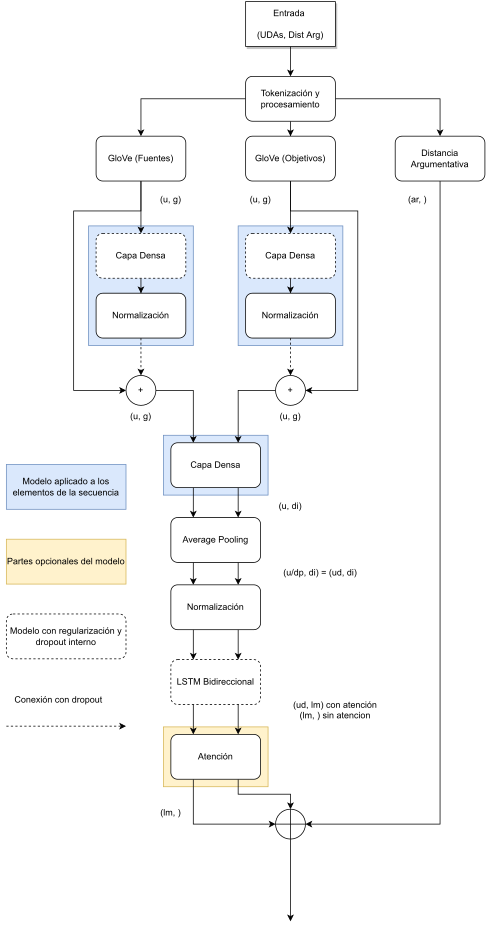
\includegraphics[scale=.6]{Graphics/Modelo_Link_Prediction1.png}
        \caption{Predictor de enlaces 1.}\label{fig:link_predictor_model1}
    \end{center}
\end{figure}
\begin{figure}[p]
    \begin{center}
        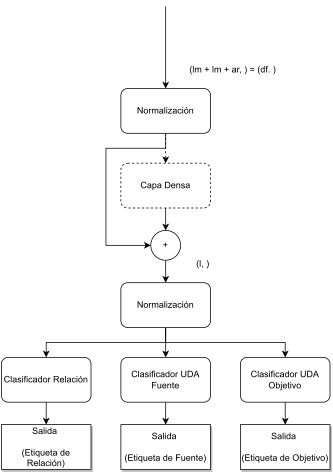
\includegraphics[scale=.4]{Graphics/Modelo_Link_Prediction2.png}
    \end{center}
    \caption{Predictor de enlaces 2.}\label{fig:link_predictor_model2}
\end{figure}

\chapter{Experimentación}\label{chapter:implementation}

En el capítulo se describe los conjuntos de datos utilizados para el entrenamiento y validación del modelo 
propuesto y cómo se construyen los conjuntos de datos en español. Se mencionan las herramientas utilizadas 
para la confección del software. Además se describe el 
proceso de experimentación y evaluación de los modelos construídos con los conjuntos de datos. Finalmente
se presentan los resultados obtenidos con los modelos al aplicarles las cartas a la dirección extraídas 
del periódico Granma. 

\section{Conjuntos de Datos}

Para el entrenamiento de los modelos propuestos se utilizaron corpus diferentes, estos
presentan esquemas de anotación distintos entre sí, difieriendo principalmente en la definición de UDA y 
las clasificaciones dadas a estas y a las relaciones. A todos los conjuntos se les proyectó al lenguaje 
español y se les realizó un aumento de datos. Como conjunto para validación fueron usadas 
una parte de las cartas a la dirección extraídas del periódico Granma.

\subsection{Ensayos Argumentativos}\label{corpus:persuasive_essays}

Este corpus [\cite{stab2017parsing}] presenta unos 402 documentos, dividido por los autores en 286 documentos para entrenamiento (70\%), 
80 para prueba (20\%) y 36 para validación (10\%). Los contenidos de estos son ensayos de estudiantes en los que 
se argumentan sobre temas como: cooperar o competir, contribuciones de la tecnología a la sociedad.
Las anotaciones de las UDAs se conforman por segmentos de textos considerados argumentativos, estos segmentos son 
clasificados en \emph{MajorClaim} (751 12\%), \emph{Claim} (1506 25\%) y \emph{Premise} (3832 63\%).
La estructura de las relaciones entre las UDAs conforman árboles en los que se tienen como raíz las 
\emph{MajorClaim} del texto. Las relaciones solo están permitidas entre \emph{Premise-Premise} y \emph{Premise-Claim}, clasificadas
en \emph{attack} (219 6\%) y \emph{support} (3613 94\%). Las relaciones entre \emph{Claim} y \emph{MajorClaim} son anotadas 
de manera diferente, por medio de 
darle a las \emph{Claim} una clasificación de si está a favor (1228) o en contra (278) de las \emph{MajorClaim} del documento.
Para el análisis de este corpus se consideraron las relaciones \emph{Claim-MajorClaim} de igual manera que las otras,
al convertir estas posiciones en relaciones. El número final con la inclusión de estas aumenta a 715 (10\%) de ataque y 
5958 (90\%) de apoyo.

\subsection{CDCP}\label{corpus:cdcp}

El corpus [\cite{niculae2017argument}] está conformado por 731 comentarios de usuarios extraídos de la web bajo el tema de 
prácticas de cobro de deudas a los consumidores (CDCP por sus siglas en inglés \emph{Consumer Debt Collection Practices}).
Las UDA se encuentran segmentadas en oraciones y todas se consideran argumentativas, estas son clasificadas en 
\emph{policy} (815 17\%), \emph{value} (2180 45\%), \emph{fact} (785 16\%), \emph{testimony} (1116 21\%) y \emph{reference} (32 1\%). 
Las relaciones se encuentran clasificadas en \emph{reason} (1352 97\%) y \emph{evidence} (73 3\%).

\subsection{AbsTRCT}

AbsTRCT [\cite{mayer2020transformer}] se compone de 500 documentos sobre el estudio de 4 enfermedades diferentes,
glaucoma, hipertensión, hepatitis b y diabetes. Las UDAs constituyen oraciones, aunque no todas son consideradas
argumentativas. Estas se clasifican en \emph{MajorClaim} (93 3\%), \emph{Claim} (993 30\%) y \emph{Premise} (2198 67\%).
Las relaciones esán representadas por tres categorías: \emph{support} (1763 85\%), \emph{partial-attack} (238 12\%) y
\emph{attack} (60 3\%).

En resumen estos datos no son grandes y contiene una gran cantidad de desbalance en sus clases.
En la Tabla \ref{table:corpus_info} se muestran los datos promedio de la composición de los diferentes corpus. 
Se observa una composición heterogenea entre estos, principalmente CDCP difiere en gran número de los demás.

\begin{table}[h!]
	\begin{center}
		\begin{tabular}{|c|c|c|c|c|} \hline
		Corpus		            & Tokens 	& Tokens argumentativos	& UDAs   & Relaciones por UDA    \\ \hline
		Ensayos Argumentativos  & 381		& 68\% 					& 35\% 	 & 1.08					 \\ \hline
		CDCP		            & 127		& 99\% 					& 97\% 	 & 0.30					 \\ \hline
		AbsTRCT	                & 371		& 50\% 					& 47\% 	 & 0.63					 \\ \hline
		\end{tabular}
	\caption{Información de promedios de los conjuntos de datos.}\label{table:corpus_info}
	\end{center}
\end{table}

\subsection{Creación de corpus en español}

\subsubsection{Aumento de datos}

A los conjuntos de datos a analizar se les realizó un aumento de datos mediante le técnica de \emph{backtranslation},
aplicándole la proyección de etiquetas de los elementos originales a los aumentados.
Esto contribuyó a duplicar la cantidad de elementos disponibles. Los resultados obtenidos al comparar los 
elementos originales con los aumentados se reflejan en la Tabla \ref{table:data_augmentation}.
Estos muestran que se logró una variación pequeña en los datos, aunque conservando la 
longitud original del texto. 

\begin{table}[h!]
	\begin{center}
		\begin{tabular}{|c|c|c|c|c|} \hline
		Corpus		            &  Jaccard	& Levenshtein	& Palabras originales / aumentadas   \\ \hline
        Ensayos Argumentativos	&  0.69		                & 96		                    & 1.00	  \\ \hline
		CDCP                    &  0.72	                    & 30		                    & 1.02	  \\ \hline
        AbsTRCT                 &  0.74		                & 86		                    & 1.04	  \\ \hline
		\end{tabular}
	\caption{Datos promedios comparando los textos originales con los aumentados.}\label{table:data_augmentation}
	\end{center}
\end{table}

\subsubsection{Proyección de corpus}

Todos los conjuntos de datos están originalmente en inglés, por lo tanto se les aplicó el algoritmo de proyección
de corpus para obtener uno en español para ser usado en el entrenamiento de los modelos. 
Para la traducción automática se utilizó los servicios de Google Translator [\cite{translateGoogle}]. Para calcular las 
alineaciones de palabras se probaron dos algoritmos, FastAlign [\cite{dyer2013fastalign}] y AwesomeAlign 
[\cite{dou2021word}]. Se observó que el primero, aunque es más rápido posee una calidad menor en los resultados,
el segundo posee una mayor calidad aunque requiere de mayor tiempo y recursos para ejecutarse. Para los experimentos
se usó finalmente AwesomeAlign. La proyección de las etiquetas fue llevada a cabo por el algoritmo propuesto 
en [\cite{eger2018cross}].

\subsection{Cartas a la dirección}

Las cartas a la dirección constituyen un segmento del periódico Granma en los cuales son publicadas
cartas enviadas por la población o empresas a dicha entidad. En general, las cartas 
presentan dudas o problemas de la población con el objetivo de obtener respuestas del organismo
asociado. Se extrajeron 2891 cartas desde el 30 de agosto del 2013 hasta el 28 de octubre del 2022. Se 
presentan aproximadamente 975000 palabras en los datos, en promedio, la cantidad de palabras por carta es de 330.
Se encontraron 874 cartas en respuesta a cartas enviadas lo que representa un 30\% del total. Se extrajeron
los comentarios asociados a las cartas, en este sentido 987 cartas no presentan comentarios y en promedio 
se realizan 2 comentarios por carta. Los textos presentan un título y un formato relativamente libre, 
aunque en las cartas de respuesta se puede observar una firma de la persona que respondió y la entidad que 
representa. Del total de cartas se seleccionaron las que fueran en respuesta a otra y también las 
cartas que fueron respondidas para tener una mayor concentración de cartas que fueran argumentativas, 
esta selección está conformada por 1702 cartas lo que representa un 59\% del total de cartas.

\section{Implementación}

La implementación de los modelos y algoritmos de procesamiento y visualización de datos se encuentran en 
un repositorio de GitHub\footnote{\url{https://github.com/luisoibarra/argument-mining}}. Esta implementación
está concebida para que se pueda extender fácilmente para el uso con otros idiomas además del inglés y el 
español. Se basa en una arquitectura de procesamiento secuencial en el cual cada paso del proceso realiza
una tarea específica y lo más desacoplada posible de las otras. Las tareas realizadas son:

\begin{itemize}
    \item Creación del corpus en un formato estándar. Dado que los corpus vienen en diferentes 
	formas, este paso se realiza para trabajar sobre una misma representación de este.
    \item Proyección del corpus de un lenguaje fuente a un lenguaje objetivo. En el caso de 
	uso del trabajo se proyecta del inglés al español.
    \begin{itemize}
        \item Traducción y alineación de oraciones.
        \item Alineación de palabras.
        \item Proyección de etiquetas.
    \end{itemize}
    \item Extracción y clasificación de UDAs.
    \item Extracción y clasificación de las relaciones entre las UDAs.
    \item Visualización de los resultados.
\end{itemize}

\subsection{Herramientas}

El lenguaje empleado para la confección del software fue python [\cite{python}], este presenta 
una gran variedad de herramientas 
para el trabajo con texto, visualización de datos y la creación de modelos de aprendizaje profundo.
Se utilizó tensorflow [\cite{tensorflow}] en su versión 2.9.2 para la construcción y entrenamiento de los modelos. 
Para el procesamiento de los textos se utilizaron nltk [\cite{nltk}] y spacy [\cite{spacy}], con estos se realizaron tareas
como la extracción de tokens y oraciones del texto, la anotación de las etiquetas POS. Se utilizaron 
ambas bibliotecas para el procesamiento debido a que, en dependencia de la situación, cada una presenta diferentes
ventajas. En el caso de nltk esta presenta algoritmos rápidos para el procesamiento de texto que no 
requieren de muchos recursos computacionales, sin embargo, estos algoritmos no están disponibles de inmediato
para otros lenguajes como el español. Spacy por su parte presenta algoritmos más certeros a costo 
de mayor tiempo de procesamiento y gasto de recursos computacionales y también presenta una cantidad de lenguajes 
disponibles mucho mayor. Para la visualización y manejo de los datos, y cálculo de métricas se utilizaron 
matplotlib [\cite{matplotlib}], pandas [\cite{pandas}] y sklearn [\cite{sklearn}]. 
Para la recolección de las cartas del periódico Granma se utilizó scrapy [\cite{scrapy}].
Como interfaz visual para el usuario se utilizó la herramienta Brat [\cite{brat}] 
(Figura \ref{fig:brat_persuasive_granma_letters}). Esta herramienta permite
la visualización y edición de las estructuras argumentativas. Dado que Brat es una página web, esta se puede
desplegar y permitir su uso online.

\begin{figure}[h!]
	\begin{center}
		% \includegraphics[scale=.4]{Graphics/persuasive_2019-01-25|informa-recursos-hidraulicos-sobre-abasto-de-agua-en-manzanillo|abasto-de-agua-en-manzanillo.png}
		\includegraphics[scale=.4, width=450pt, height=250pt]{Graphics/persuasive_2019-03-22|inconformidad-con-la-chequera.png}
		\caption{Visualización con Brat de las estructuras argumentativas.}\label{fig:brat_persuasive_granma_letters}
	\end{center}
\end{figure}

\subsection{Formato Estándar}

El formato estándar creado es basado en el esquema de anotación CoNLL, en este se anotan todos los aspectos 
relavantes para las tareas a relizar. La segmentación de las UDAs son representadas por las anotaciones 
BIO o BIOES en cada palabra, en adición, las clasificaciones de estas son anotadas al adicionar el nombre 
de esta separada por un guión. Las relaciones son anotada auxiliándose de la distancia argumentativa, estas 
son agregadas al anotar el tipo de relación con su respectiva distancia ambas separadas por un guión. A 
continuación se muestran ejemplos de este formato:

\begin{itemize}
	\item Inicio de UDA con dos relaciones: $atletas \quad B-Claim-attacks--1-attacks-12$
	\item UDA intermedia con una relación: $contribuye \quad I-Premise-attacks-5$
	\item Elemento fuera de una UDA: $análisis \quad O$
\end{itemize}

\section{Experimentación}

Para realizar la selección del modelo se utilizó el corpus de Ensayos Argumentativos. Con este se ajustaron
las arquitecturas e hiperparámetros de los modelos propuestos. La mejor combinación de estos fue utilizada 
para el entrenamiento de los corpus restantes. Finalmente los modelos fueron utilizados para anotar las cartas 
a la dirección. 

\subsection{Hardware}

Gran parte del procesamiento se llevo a cabo en una computadora $i5$ con $8GB$ de RAM ampliada con $4GB$ de memoria 
\emph{swap} [\cite{swap}], aunque se requirió el uso de la plataforma \textbf{Colab} [\cite{colab}] para 
el entrenamiento de algunos modelos por falta de recursos locales.

\subsection{Segmentador de UDA}

En el entrenamiento del segmentador de UDA se hicieron variaciones en la arquitectura propuesta con respecto a la
presencia o no de las siguiente componentes:

\begin{itemize}
    \item Atributos de POS en la entrada del algoritmo.
    \item Atributos extraídos por la CNN de la palabra.
    \item Atributos features extraídos por la LSTM bidireccional de la palabra.
    \item Conexiones residuales.
    \item Capa densa final.
    \item Capas de normalizaciones.
\end{itemize}

De las posibles combinaciones se presentaron 4 candidatos:

\begin{table}[h!]
	\begin{center}
		\begin{tabular}{|c|c|c|c|c|c|c|} \hline
		Modelos 	& POS       & Char-CNN  & Char-LSTM & Res       & Norm      & Densa  \\ \hline
		Modelo1		& $\times$	& $\times$    & $\times$    & $\times$	& $\times$    & $\times$ \\ \hline
		Modelo2		& $\times$	& $\checkmark$    & $\checkmark$    & $\checkmark$	& $\checkmark$    & $\times$ \\ \hline
		Modelo3		& $\checkmark$	& $\checkmark$    & $\checkmark$    & $\checkmark$	& $\checkmark$    & $\times$ \\ \hline
		Modelo4		& $\checkmark$	& $\checkmark$    & $\checkmark$    & $\checkmark$	& $\checkmark$    & $\checkmark$ \\ \hline
		\end{tabular}
	\caption{Variantes de arquitectura de los modelos de segmentación de UDA.}\label{table:segmenter_architecture_table}
	\end{center}
\end{table}

En la figura (\ref{fig:segmenter_model_loss}) se observan las diferentes curvas de aprendizaje de los modelos 
probados. Se muestra la rápida convergencia de los modelos con conexiones residuales y normalizaciones.
Se muestra también la tendencia al sobreajuste en el entrenamiento entre los pasos 17-20, en donde se detiene el 
entrenamiento para evitar el crecimiento del error de generalización.

\begin{figure}[h!]
	\begin{center}
		\begin{center}
			\includegraphics[scale=.7]{Graphics/persuasive_essays_all_linked_crf_loss.png}
        \end{center}
	    \caption{Pérdida de los modelos segmentadores.}\label{fig:segmenter_model_loss}
	\end{center}
\end{figure}

Las métricas \%F1 muestran que los modelos 1 y 2 presentan un desempeño menor que los 3 y 4. 
Se muestra un ligero aumento de 1\% en las 50\%F1 en el modelo 4 con respecto 
al modelo 3, aunque las métricas de F1 en el 3 superan a las de 4. Se considera que la 
segmentación como tarea principal, por lo que se selecciona como mejor modelo al 4 (Figura \ref{fig:test_segmenter_model_metrics}).

\begin{figure}[h!]
	\begin{center}
		\includegraphics[scale=.4]{Graphics/persuasive_essays_all_linked_components.png}
		\includegraphics[scale=.4]{Graphics/persuasive_essays_all_linked_macro_micro_metrics.png}
	    \caption{Métricas del conjunto de pruebas de los modelos segmentadores.}\label{fig:test_segmenter_model_metrics}
	\end{center}
\end{figure}

El modelo seleccionado fue usado en el entrenamiento de los demás conjuntos de datos obteniendo los resultados mostrados
en Tabla \ref{table:test_metrics_segmenter} y Tabla \ref{table:test_bioes_metrics_segmenter}.

\begin{table}[h!]
	\begin{center}
		\begin{tabular}{|c|c|c|c|c|c|} \hline
        Corpus		            & F1 Ponderado  & Macro F1	& \emph{Accuracy} & 100\%F1 & 50\%F1  	   \\ \hline
        Ensayos Argumentativos  & .76           & .56 		& .77		      & .72	    & .83	       \\ \hline
        CDCP		            & .65           & .45 		& .66		      & .61	    & .68	       \\ \hline
        AbsTRCT	                & .86           & .50 		& .87		      & .61	    & .75	       \\ \hline
        \end{tabular}
	\caption{Métricas de las pruebas del segmentador de UDA.}\label{table:test_metrics_segmenter}
	\end{center}
\end{table}
\begin{table}[h!]
	\begin{center}
		\begin{tabular}{|c|c|c|c|c|c|} \hline
        Corpus		            & F1 Ponderado  & Macro F1 & \emph{accuracy} & 100\%F1 &  50\%F1   \\ \hline
        Ensayos Argumentativos  & .89           & .82	   & .89             & .81	   & .94 	   \\ \hline
        CDCP		            & .95           & .56	   & .96	         & .82	   & .93 	   \\ \hline
        AbsTRCT	                & .90           & .79	   & .91	         & .66	   & .82 	   \\ \hline
        \end{tabular}
	\caption{Métricas BIOES de las pruebas del segmentador de UDA.}\label{table:test_bioes_metrics_segmenter}
	\end{center}
\end{table}

\subsection{Predictor de Enlaces}

Para el modelo se realizó un voto conjunto del ensamblado de 3 modelos, dado que en el entrenamiento se 
está basado en la aleatoriedad se entrenan los modelos con los mismos datos obteniendo inferencias no
necesariamente iguales.
Para la selección del modelo se entrenaron diferentes variantes de arquitecturas y hiperparámetros, y 
al igual que en el segmentador de UDAs se realizó la selección del modelo que mejor se desempeñó en 
el conjunto de datos de Ensayos Argumentativos. De las variaciones surgieron las siguientes propuestas:

\begin{table}[h!]
	\begin{center}
		\begin{tabular}{|c|c|c|c|c|c|c|} \hline
		Modelos  & Atención      & Pooling  & \emph{Dropout}   & Tasa de aprendizaje & Paciencia & Devolver mejores     \\ \hline
		Modelo1	 & $\times$	     &  5       & .5               & .0015               & 10	      & $\checkmark$        \\ \hline
		Modelo2	 & $\times$	 	 & 10       & .1               & .003                & 5	      & $\times$            \\ \hline
		Modelo3	 & $\checkmark$	 &  1       & .1               & .003                & 5	      & $\times$            \\ \hline
		Modelo4	 & $\checkmark$	 &  1       & .5               & .0015               & 10	      & $\checkmark$        \\ \hline
		\end{tabular}
	\caption{Variantes de arquitectura de los modelos de predicción de enlaces.}\label{table:link_predictor_architecture_table}
	\end{center}
\end{table}

Las curvas de aprendizaje del proceso de entrenamiento de los modelos (Figura \ref{fig:link_prediction_model_loss}) 
muestran un nivel de sobreajuste 
elevado que disminuyen cuando el \emph{dropout} aumenta. Además se observan valores de pérdida elevados lo que significa 
que el modelo le cuesta ajustarse de manera satisfactoria a los datos.

\begin{figure}[h!]
	\begin{center}
		\includegraphics[scale=.7]{Graphics/persuassive_essays_all_linked_link_prediction_loss_model_1.png}
	    \caption{Curvas de aprendizaje de los modelos de predicción de enlaces.}\label{fig:link_prediction_model_loss}
	\end{center}
\end{figure}

Las métricas obtenidas por las diferentes versiones de los modelos 
(Figura \ref{fig:link_prediction_model_metrics}) 
muestran que el modelo 2 constituye una opción ligeramente superior en lo correspondiente a 
predicción de enlace a los otros modelos. Esos hiperparámetros
fueron utilizados para el entrenamiento con los demás conjuntos de datos.

\begin{figure}[h!]
	\begin{center}
		\includegraphics[scale=.4]{Graphics/persuasive_essays_all_linked_all_relation_f1_scores.png}
		\includegraphics[scale=.4]{Graphics/persuasive_essays_all_linked_all_relation_accuracy.png}
	\end{center}
	\begin{center}
		\includegraphics[scale=.4]{Graphics/persuasive_essays_all_linked_all_relation_linked.png}
	    \caption{Métricas F1 de la clasificación de enlace (izquierda), \emph{accuracy} (derecha) y
				 F1 de la predicción de enlace (abajo) de los modelos de predicción de enlaces.}\label{fig:link_prediction_model_metrics}
	\end{center}
\end{figure}

En el entrenamiento del modelo en los demás cojuntos de datos se los resultados siguientes:

\begin{table}[h!]
	\begin{center}
		\begin{tabular}{|c|c|c|c|c|} \hline
        Corpus		            & Macro F1 & \emph{Accuracy} & Macro F1 Enlace  & \emph{Accuracy} Enlace  \\ \hline
        Ensayos Argumentativos  & .33	   & .57             & .68	    		& .75	    		  	  \\ \hline
        CDCP		            & .37	   & .63	         & .79	    		& .68	    		  	  \\ \hline
        AbsTRCT	                & .39	   & .61	         & .83	    		& .74	    		  	  \\ \hline
        \end{tabular}
	\caption{Métricas de predicción de relaciones de las pruebas del predictor de enlace.}\label{table:test_relation_metrics_link_predictor}
	\end{center}
\end{table}

\begin{table}[h!]
	\begin{center}
		\begin{tabular}{|c|c|c|c|} \hline
        Corpus		            & F1 Macro  & \emph{Accuracy} \\ \hline
        Ensayos Argumentativos  & .48       & .60             \\ \hline
        CDCP		            & .26       & .52	         \\ \hline
        AbsTRCT	                & .51       & .79	         \\ \hline
        \end{tabular}
	\caption{Métricas de predicción de fuente de las pruebas del predictor de enlace.}\label{table:test_source_metrics_link_predictor}
	\end{center}
\end{table}

\begin{table}[h!]
	\begin{center}
		\begin{tabular}{|c|c|c|c|} \hline
        Corpus		            & Macro F1 & \emph{Accuracy} \\ \hline
        Ensayos Argumentativos  & .52	   & .57             \\ \hline
        CDCP		            & .36	   & .54	         \\ \hline
        AbsTRCT	                & .53	   & .81	         \\ \hline
        \end{tabular}
	\caption{Métricas de predicción de objetivo de las pruebas del predictor de enlace.}\label{table:test_target_metrics_link_predictor}
	\end{center}
\end{table}

\subsection{Acoplamiento de los modelos}

Dado que la clasificación de UDAs es hecha tanto en el segmentador como en el predictor de enlaces es necesaria 
la selección de cómo se va a desambiguar esta clasificación. En caso de seleccionar el predictor de enlaces como 
clasificador final, surgen varias cuestiones como por ejemplo, las UDAs pueden tomar varias clasificaciones o el
predictor no toma el contexto del texto completo en la clasificación. Aunque la primera puede ser corregida
mediante la selección de la clase más votada o algún otro criterio, la segunda presenta un mayor problema. Por
esto es seleccionada la clasificación del segmentador como etiqueta final para las UDAs y el predictor es usado para 
la tarea de extracción y clasificación de relaciones.

\subsection{Comparación con estados del arte}

Las comparaciones se realizan por conjuntos de datos y se muestran las 
métricas indicadas por los autores de cada propuesta. Cada corpus y propuesta 
presenta características únicas que hacen que comparaciones directas sean 
difíciles de realizar, por lo tanto la información brindada muestra una comparación 
cualitativa y no cuantitativa en la mayoría de los casos. 

Una de las principales dificultades está dada por el hecho de que las métricas calculadas son de la versión proyectada
al español, lo cual contribuye a variaciones en las etiquetas finales debido al lenguaje mismo 
o a errores en el proceso. Otros ejemplos en la dificultad de comprarar las métricas se encuentra
en los enfoques tomados por las investigaciones anteriores a la hora de realizar las tareas.
En algunos casos la segmentación se presenta como una tarea de clasificación BIO, o simplemente 
se separan por oraciones y las clasifican en argumentativas o no. En el aspecto de clasificación
de las UDAs se emplean métodos como su clasificación independiente luego de ser extraída o su modelación
conjunta con la segmentación. En la extracción y clasificación de relaciones se observan técnicas de 
optimización de problemas enteros, clasificación por SVM o también probando los posibles enlaces dos 
a dos independientemente.

En la comparación de métodos se seleccionaron seis métricas que evalúan las diferentes 
tareas de la EA. La métrica BIOES F1 se refiere 
a la Macro F1 de la clasificación de las etiquetas BIOES, esta constituye una medida
que califica la tarea de segmentación de UDAs en el texto. La métrica Clas UDA F1 es 
calculada como la Macro F1 de las etiquetas BIOES junto con las etiquetas del tipo de 
UDA, medida que evalúa la tarea de clasificación de las UDAs. Rel Pred F1 es la medida 
Macro F1 de la predicción de enlaces y Rel Clas F1 la de la clasificación, estas 
son calculadas tomando en cuenta todos los pares seleccionados para el conjunto de 
datos. En la comparación $\checkmark$ significa que son directamente comparables,
$*$ que el método de comparación es el mismo pero no son usados los mismos 
elementos para calcular la métrica y $\times$ que la métrica no se encontraba disponible.

\begin{table}[h!]
	\begin{center}
		\begin{tabular}{|c|c|c|c|c|c|} \hline
		Corpus		            & Propuesto  & \cite{stab2017parsing} & \cite{niculae2017argument} & \cite{galassi2021deep} \\ \hline
		BIOES F1 				& .82   	 & .85 $\checkmark$		  & $\times$        	       & $\times$				\\ \hline
		Clas UDA F1		        & .56	     & .82        			  & .77	    			       & .53					\\ \hline
		Rel Pred F1 			& .68   	 & .58        			  & .60			    	       & .36 *				   	\\ \hline
		Rel Clas F1 			& .33   	 & .70        			  & $\times$	    	       & .18 *				   	\\ \hline
		\end{tabular}
	\caption{Métricas comparativas de Ensayos Persuasivos.}\label{table:comparative_test_essays_f1_metrics_segmenter}
	\end{center}
\end{table}
\begin{table}[h!]
	\begin{center}
		\begin{tabular}{|c|c|c|c|c|c|} \hline
		Corpus		            & Propuesto  & \cite{niculae2017argument} & \cite{galassi2021deep}  \\ \hline
		BIOES F1 				& .56  	 	 & $\times$        	       	  & $\times$				\\ \hline
		Clas UDA F1		        & .45	     & .73 				 		  & .79					   	\\ \hline
		Rel Pred F1				& .68   	 & .27			    	      & .30	*			   	    \\ \hline
		Rel Clas F1				& .37   	 & $\times$	    	          & .15	*			   	    \\ \hline
		\end{tabular}
	\caption{Métricas comparativas de CDCP.}\label{table:comparative_test_cdcp_f1_metrics_segmenter}
	\end{center}
\end{table}
\begin{table}[h!]
	\begin{center}
		\begin{tabular}{|c|c|c|c|c|c|} \hline
		Corpus		            & Propuesto  & \cite{mayer2020transformer} & \cite{galassi2021deep} \\ \hline
		BIOES F1 				& .79   	 & $\times$   				   & $\times$				\\ \hline
		Clas UDA F1		        & .50	     & .88	$\checkmark$		   & .91					\\ \hline
		Rel Pred F1 			& .74   	 & $\times$	   				   & .54 *				   	\\ \hline
		Rel Clas F1 			& .39   	 & .66  *	   				   & .70 *				   	\\ \hline
		\end{tabular}
	\caption{Métricas comparativas de AbsTRCT.}\label{table:comparative_test_abstrct_f1_metrics_segmenter}
	\end{center}
\end{table}

\section{Validación}

Dado que las estructuras argumentativas varían en su forma en cada corpus es complejo realizar un método que evalúe de forma 
justa los resultados obtenidos por los diferentes modelos de manera conjunta. Una variante sería anotar las cartas 
con los esquemas argumentativos presentes en los conjuntos de datos, esto constituye una labor en la que se requiere
personal experto y previo estudio y preparación, además de tiempo. El proceso que se lleva a cabo para realizar la 
validación consiste en un análisis cualitativo realizado a criterio del autor. Para esto se seleccionaron 15 pares 
de cartas, respondidas y en respuesta. Cada uno de estas 30 cartas fueron anotadas por los modelos entrenados en cada 
conjunto de datos y se realizó el análisis de calidad correspondiente. Los puntos por los que se llevó a cabo el análisis
se resumen en los siguientes:

\begin{itemize}
	\item ¿La UDA se extrajo correctamente?
	\item ¿La UDA se clasificó correctamente?
	\item ¿La relación se extrajo correctamente?
	\item ¿La relación se clasificó correctamente?
\end{itemize}

% \begin{itemize}
% 	\item Muchos falsos positivos en la predicción de enlaces, debido a la manera en la manera componente a componente que 
% 	se hacen
% 	\item En los textos en donde la segmentación es por oraciones, los puntos relacionados a otra acción que 
% 	no sea separar oraciones son seleccionados como separadores.
% 	\item La segmentación, se queda corta o larga?
% \end{itemize}

\subsection{Análisis Ensayos Argumentativos}

% \begin{figure}[h!]
% 	\begin{center}
% 		\includegraphics[scale=.4]{Graphics/persuasive_2019-01-25|informa-recursos-hidraulicos-sobre-abasto-de-agua-en-manzanillo|abasto-de-agua-en-manzanillo.png}
% 		\includegraphics[scale=.4]{Graphics/persuasive_2019-03-22|inconformidad-con-la-chequera.png}
% 	    \caption{A}\label{fig:persuasive_granma_letters}
% 	\end{center}
% \end{figure}

Los ensayos argumentativos presentan una anotación de UDAs a un nivel de unidades de texto que pueden ser 
más pequeñas que oraciones y clasifican estas en las clases MajorClaim (MC), Claim (C) y Premise (P). Las 
relaciones se clasifican en de \emph{supports} y \emph{attacks}. 

En general se observa que se presentan problemas en la segmentación de UDAs debido al formato y dominio del texto.
Las cartas presentan una estrutura en donde al final se realiza una firma poniendo información acerca del remitente,
esta estructura no contribuye a la argumentación, pero el modelo en varias ocasiones detecta componentes en estas. 
Además de estos problemas de la estructura característica de la carta se encuentran otros problemas. Entre los más 
encontrados se observa la extracción de supuestas UDAs que en su contenido no se encuentra un componente argumentativo, 
generalmente estos elementos, si se expanden, pueden lograr establecer una mejor UDA.

Ejemplos malos:
\begin{itemize}
	\item \text{} [años de explotación y]$_{MC}$ 
	: Muy corto y no informativo. % 2019-01-25|informa-recursos-hidraulicos-sobre-abasto-de-agua-en-manzanillo|abasto-de-agua-en-manzanillo.txt.conll.link.conll.ann
	\item \text{} [en cada uno de los establecimientos de nuestra Cadena de Tiendas]$_{MC}$ 
	: Incompleto, mejora incorporando elementos de la izquierda (No a todos los productos con próxima fecha de vencimiento se le aplica rebaja de precios). % 2018-12-07|responde-trd-caribe-al-consumidor|a-proposito-de-la-proteccion-al-consumidor.txt.conll.link.conll.ann
	\item \text{} [Director División Grandes Centros]$_{MC}$ [trd Caribe]$_{C}$ 
	: Mala clasificación y segmentación. %  2018-12-07|responde-trd-caribe-al-consumidor|a-proposito-de-la-proteccion-al-consumidor.txt.conll.link.conll.ann
	\item \text{} [Esperamos lo antes posible una solución]$_{P}$ 
	: En contexto, no contiene información que lo haga premisa % 2018-10-05|abasto-de-agua-en-manzanillo.txt.conll.link.conll.ann
	\item \text{} [no podemos permitir]$_{C}$ 
	: No establece una \emph{claim} % 2017-06-30|inass-reconoce-razon-de-ramiro-castellanos-por-inconformidad-con-trato-de-especialista-de-las-tunas|pregunta-quien-le-paga-su-jubilacion.txt.conll.link.conll.ann
\end{itemize}

Ejemplos buenos:
\begin{itemize}
	\item \text{} [no se le puede volver a despachar , tiene que ver a la administración ( si está ahí en ese momento ) , 
	si no , regresar al día siguiente para que se le acredite lo sucedido]$_{MC}$ % 2021-02-26|inconvenientes-con-tarjetas-de-combustible-en-moneda-nacional.txt.conll.link.conll.ann
	\item \text{} [administración de la emi Yuri Gagarin desde inicios de la confección del expediente para 
	mi jubilación , no contempló el salario obtenido por pluriempleo]$_{MC}$ % 2019-03-22|inconformidad-con-la-chequera.txt.conll.link.conll.ann
	\item pudiese [contribuir al ahorro de agua y la prestación de un mejor servicio]$_C$ % 2018-10-05|abasto-de-agua-en-manzanillo.txt.conll.link.conll.ann
	\item \text{} [es que estamos limitados de este servicio , y no desde hace un tiempo , es que nunca lo hemos tenido]$_P$ % 2018-05-18|sin-cobertura-en-guara-mayabeque.txt.conll.link.conll.ann
	\item \text{} [el número de carné de identidad que se encontraba en dicha base de datos correspondía a otra persona que
	fue reportada como fallecida]$_P$ % 2017-06-30|inass-reconoce-razon-de-ramiro-castellanos-por-inconformidad-con-trato-de-especialista-de-las-tunas|pregunta-quien-le-paga-su-jubilacion.txt.conll.link.conll.ann
\end{itemize}

Las relaciones anotadas por el modelo tienden a contener una gran cantidad de falsos positivos, además
dado que este conjunto de datos posee un gran desbalance en las etiquetas de las relaciones favoreciendo 
estas a las de \emph{supports}, el modelo no fue capaz de realizar anotaciones de \emph{attacks}, tanto en 
el conjunto de original de pruebas como en las cartas.

\subsection{Análisis CDCP}

% \begin{figure}[h!]
% 	\begin{center}
% 		\includegraphics[scale=.4]{Graphics/cdcp_2019-01-25|informa-recursos-hidraulicos-sobre-abasto-de-agua-en-manzanillo|abasto-de-agua-en-manzanillo.png}
% 		\includegraphics[scale=.4]{Graphics/cdcp_2019-03-22|inconformidad-con-la-chequera.png}
% 	    \caption{A}\label{fig:cdcp_granma_letters}
% 	\end{center}
% \end{figure}

CDCP realiza la segmentación de UDAs en la mayoría de las situaciones al separarlas por oraciones 
(solamente el 1\% de los tokens se encuentran fuera de una UDA),
estas son clasificadas en \emph{testimony} (T), \emph{fact} (F), \emph{policy} (P), \emph{reference} (R)
y \emph{value} (V). Las relaciones presentan dos tipos de relaciones \emph{evidences} and \emph{reasons}.

Los errores más comunes cometidos en la segmentación dado el esquema utilizado provienen de el uso 
de signos de puntuación no representando un cambio de oración, en estos casos se separa las UDA. También
existen errores de clasificación incorrecta, de por ejemplo \emph{testimony} que podrían ser \emph{fact}.

Ejemplos malos:
\begin{itemize}
	\item \text{} [\dots Bayamo , km 1 No .]$_T$ [30 A ( interior ) , \dots]$_T$ 
	: Uso del \textbf{.} para abreviar número se toma como separador de UDA. % 2019-01-25|informa-recursos-hidraulicos-sobre-abasto-de-agua-en-manzanillo|abasto-de-agua-en-manzanillo.txt.conll.link.conll.ann
	\item \text{} [\dots , desde el 1ro .]$_T$ [de marzo \dots]$_T$ 
	: Uso del \textbf{.} para abreviar primero se toma como separador de UDA. % 2019-05-24|le-retribuyen-la-diferencia-reclamada-de-su-pension|inconformidad-con-la-chequera.txt.conll.link.conll.ann
	\item \text{} [Junto a la misiva se le entregó al Inass certificados de salarios devengados y las tarjetas sn2-25 .]$_T$ 
	: Se clasifica mejor como \emph{fact}. % 2019-03-22|inconformidad-con-la-chequera.txt.conll.link.conll.ann
	\item \text{} [Caridad Real Gutiérrez , Jefe de Trámites y Pensiones , Inass .]$_T$ 
	: Firma de la carta como elemento argumentaivo. % 2019-05-24|le-retribuyen-la-diferencia-reclamada-de-su-pension|inconformidad-con-la-chequera.txt.conll.link.conll.ann
\end{itemize}

Ejemplos buenos:
\begin{itemize}
	\item \text{} [En el 2017 se colocaron tuberías de 200 , 160 y 110 mm , quedando no concluido y de 
	continuidad para el 2018 se situó un financiamiento para construcción de registros y colocación de 
	válvulas y ventosas .]$_F$ % 2019-01-25|informa-recursos-hidraulicos-sobre-abasto-de-agua-en-manzanillo|abasto-de-agua-en-manzanillo.txt.conll.link.conll.ann
	\item \text{} [Mi jubilación comenzó el 29 de febrero de 2016 , no el 29 de febrero de 2017 .]$_T$ % 2019-03-22|inconformidad-con-la-chequera.txt.conll.link.conll.ann
	\item \text{} [No se sabe cuánto queda , lo que obliga al cliente a estar haciendo cuentas constantemente .]$_F$ % 2021-05-07|servicentros-operan-diversos-medios-de-pago-electronicos|inconvenientes-con-tarjetas-de-combustible-en-moneda-nacional.txt.conll.link.conll.ann
\end{itemize}

Las relaciones presentes disminuyen en cantidad en comparación con lo visto en los textos anotados con el modelo 
entrenado con Ensayos Argumentativos. Prevaleciendo las relaciones de \emph{reasons}. A consideración del autor,
la cantidad de los falsos positivos son menores que el modelo de Ensayos Argumentativos.

\subsection{Análisis AbsTRCT}

% \begin{figure}[h!]
% 	\begin{center}
% 		\includegraphics[scale=.4]{Graphics/abstrct_2019-01-25|informa-recursos-hidraulicos-sobre-abasto-de-agua-en-manzanillo|abasto-de-agua-en-manzanillo.png}
% 		\includegraphics[scale=.4]{Graphics/abstrct_2019-03-22|inconformidad-con-la-chequera.png}
% 		\caption{A}\label{fig:abstrct_granma_letters}
% 	\end{center}
% \end{figure}

El conjunto de datos presenta un estilo de segmentación de UDAs en donde se anotan 
secciones de textos m'as grandes que en Ensayos Argumentativos, aunque no necesariamente 
todas las oraciones o la oración completa es considerada argumentativa. 
Estas se clasifican igual que Ensayos Argumentativos, aunque 
en este conjunto de datos se presenta un desbalance de etiquetas grande, favoreciendo 
a las \emph{Premise} y las \emph{Claim}, dejando sin representación casi a \emph{MajorClaim}
(menor del 1\% de las etiquetas BIOES), lo que trajo como consecuencia que el modelo no fuera 
capaz de diferenciar este tipo de UDA. Las relaciones se presentaron como \emph{partial-attack},
\emph{attack} y \emph{support}, influenciadas también por la poca cantidad de relaciones de \emph{attack}.

En la clasificación de UDAs se evidencia una gran cantidad de \emph{Premise}

Ejemplos malos:
\begin{itemize}
	\item \text{} [\dots Calle 14 , apto .]$_P$ [4 entre Zapata y 23 , \dots]$_T$ 
	: Uso del \textbf{.} para abreviar número se toma como separador de UDA. % 2017-07-07|parque-en-pleno-deterioro-en-plaza.txt.conll.link.conll.ann
	\item \text{} [, Director División Grandes Centros trd Caribe .]$_C$ 
	: Mala clasificacion con mala segmentación y detección de \emph{claim} en firma de carta. 
\end{itemize}

Ejemplos buenos:
\begin{itemize}
	\item \text{} [Esta situación pudo haberse evitado y no podemos permitir que hechos como este ocurran pues , 
	empañan la imagen de la institución que está destinada a brindar un servicio con calidad a la población en 
	general y en especial a los jubilados y pensionados .]$_P$ % 2017-06-30|inass-reconoce-razon-de-ramiro-castellanos-por-inconformidad-con-trato-de-especialista-de-las-tunas|pregunta-quien-le-paga-su-jubilacion.txt.conll.link.conll.ann
	\item \text{} [Esta respuesta considera sin razón la preocupación de un lector , 
	¿así debe terminar la inquietud de un ciudadano , que confía en las instituciones con que cuenta la 
	sociedad para enfrentar sus problemas ?]$_C$ % 2017-05-12|cimex-se-dirige-a-limitado-fisico-motor|llamado-a-evaluar-situacion-de-piezas-y-baterias-para-equipos-motorizados-de-discapacitados.txt.conll.link.conll.ann
\end{itemize}

Las relaciones tienen la menor cantidad de elementos de los otros conjuntos de datos, proliferando
las relaciones de \emph{support}. En las clasificadas como \emph{partial-attack} se evidenció, a 
consideración del autor, una baja precisión. Por ejemplo 
[\emph{cierto que la responsabilidad es de todos , pero la institucional es de la Dirección de Comunales .}]
ataca a [\emph{Antonio Blanco , Director de Servicios Comunales Plaza ,}].

\subsection{Resultados}

Se considera que el conjunto de datos CDCP se ajusta mejor a las características de las Cartas 
a la Dirección. Este presenta orígenes similares, es contenido generado por usuarios en una plataforma
web, y por lo tanto presenta un conjunto de etiquetas de UDAs que se ajustan más a lo observado 
en las cartas. También las cartas presentan un alto contenido argumentativo, por lo que marcar 
todas las oraciones como argumentativas no constituye una fuente grande de errores, aunque esta 
parte puede ser mejorada. Una desventaja de este esquema sobre otros es la carencia de una 
clasificación de las relaciones que implique un ataque, aunque esto se cubre con el hecho de 
que en los conjuntos en donde existen estas los resultados son bastante pobres. La cantidad 
y calidad de relaciones, aunque tiene bastante espacio para mejorar, es aceptable dada la dificultad 
del problema en EA.

Con CDCP se obtiene una visión general de la argumentación, aunque si se desea obtener algo 
más específico podría considerarse el modelo de Ensayos Argumentativos. La ventaja de este 
modelo en la extracción y clasificación de UDA es que utiliza un conjunto de etiquetas que 
podría considerarse universal en la argumentación y además reduce el espacio de búsqueda de 
oraciones a segmentos de palabras, aunque estos puedan estar sujetos a errores. 

La versión de AbsTRCT constituye el modelo con menor rendimiento. La clasificación
de UDAs presenta una gran desproporción hacia \emph{Premise} dejando muchas \emph{Claim}
sin ser conrrectamente clasificadas. Sobre las relaciones muestra un nivel muy bajo de 
relaciones por documento, en relación a las que se podrían formar.


\backmatter

\begin{conclusions}

% TODO Como se cumplieron los objetivos de la introduccion y para que sirve lo que hice

En el trabajo se implement'o un algoritmo con el cual se hace posible la extracción de las estructuras
argumentativas de textos 


\end{conclusions}

\begin{recomendations}
    Recomendaciones

    \begin{enumerate}
        \item Usar metodos de Graph Neural Networks para modelar las relaciones entre las UDA. (Actualmente las relaciones extraídas son independientes)
        \item Ajustar (Tune) awesome-align con inglés-español.
        \item Usar otros embeddings para la representación de palabras (BERT, SciBERT, RoBERTa).
        \item Desplegar un servidor Brat para socializar los resultados y permitir que los investigadores perfeccionen las anotaciones.
        \item Validación externa con lingüistas que permitan generalizar el uso del modelo.
    \end{enumerate}
\end{recomendations}

\printbibliography[heading=bibintoc]

%\begin{thebibliography}{99}
%
%\bibitem{texbook}
%Donald E. Knuth (1986) \emph{The \TeX{} Book}, Addison-Wesley Professional.
%
%
%\end{thebibliography}
%\begin{document}
%\bibliography{Bibliography}
%
%\end{document}

\end{document}